\chapter{Extense report - Fieldwork data analysis}
\label{chapter:Extense_fieldwork_analysis}

This appendix accommodates a complete overview in fieldwork data analysis. Each location specific dataset is analysed by a distinction in method (analytical Theis's method (single layer), \texttt{Fmin} and TTim \texttt{Calibrate})) and theoretical model (single layer, double layer, partially penetrating double layer). In the TTim analysis an additional distinction is made between analysis by the use of (a) actual borehole storage and no well resistance, (b) optimal borehole storage and no well resistance, (c) actual borehole storage and optimal well resistance, (d) optimal borehole storage and optimal well resistance. Result is the location specific dataset analysis subjected to 25 different approaches; analytical (1x), Fmin-RMSE (4x3 = 12x) and TTim Calibrate (4x3 = 12x). Outcomes in geohydrological parameter values can be found in the tables and figures below.   

\clearpage\section{Bingo - overview}
\label{sec:Bingo_overview}

\begin{figure}[h!]
	\centering
	\begin{subfigure}[b]{0.65\linewidth}
		\centering\includegraphics[width=\linewidth]{Bingo_1lay_fmin}
		\captionsetup{justification=centering}		
		\caption{\label{fig:Bingo_1lay_fmin}}
		\end{subfigure}\vfill
	\begin{subfigure}[b]{0.65\linewidth}
		\centering\includegraphics[width=\linewidth]{Bingo_1lay_cal}
		\captionsetup{justification=centering}		
		\caption{\label{fig:Bingo_1lay_cal}}
		\end{subfigure}
	\captionsetup{justification=centering}	
	\caption{Bingo single layer fieldwork data analysis by the optimization (\subref{fig:Bingo_1lay_fmin}) fmin-RMSE method and (\subref{fig:Bingo_1lay_cal}) TTim calibration method} 
	\label{fig:Bingo_1lay_analysis}
\end{figure} 

\begin{figure}[h!]
	\centering
	\begin{subfigure}[b]{0.65\linewidth}
		\centering\includegraphics[width=\linewidth]{Bingo_2lay_fmin}
		\captionsetup{justification=centering}		
		\caption{\label{fig:Bingo_2lay_fmin}}
		\end{subfigure}\vfill
	\begin{subfigure}[b]{0.65\linewidth}
		\centering\includegraphics[width=\linewidth]{Bingo_2lay_cal}
		\captionsetup{justification=centering}		
		\caption{\label{fig:Bingo_2lay_cal}}
		\end{subfigure}
	\captionsetup{justification=centering}	
	\caption{Bingo double layer fieldwork data analysis by the optimization (\subref{fig:Bingo_2lay_fmin}) fmin-RMSE method and (\subref{fig:Bingo_2lay_cal}) TTim calibration method} 
	\label{fig:Bingo_2lay_analysis}
\end{figure} 

\begin{figure}[h!]
	\centering
	\begin{subfigure}[b]{0.65\linewidth}
		\centering\includegraphics[width=\linewidth]{Bingo_3lay_fmin}
		\captionsetup{justification=centering}		
		\caption{\label{fig:Bingo_3lay_fmin}}
		\end{subfigure}\vfill
	\begin{subfigure}[b]{0.65\linewidth}
		\centering\includegraphics[width=\linewidth]{Bingo_3lay_cal}
		\captionsetup{justification=centering}		
		\caption{\label{fig:Bingo_3lay_cal}}
		\end{subfigure}
	\captionsetup{justification=centering}	
	\caption{Bingo partially penetrating double layer fieldwork data analysis by the optimization (\subref{fig:Bingo_3lay_fmin}) fmin-RMSE method and (\subref{fig:Bingo_3lay_cal}) TTim calibration method} 
	\label{fig:Bingo_3lay_analysis}
\end{figure} 

\clearpage

\begin{figure}[h!]
	\centering
	\begin{subfigure}[b]{\linewidth}
		\centering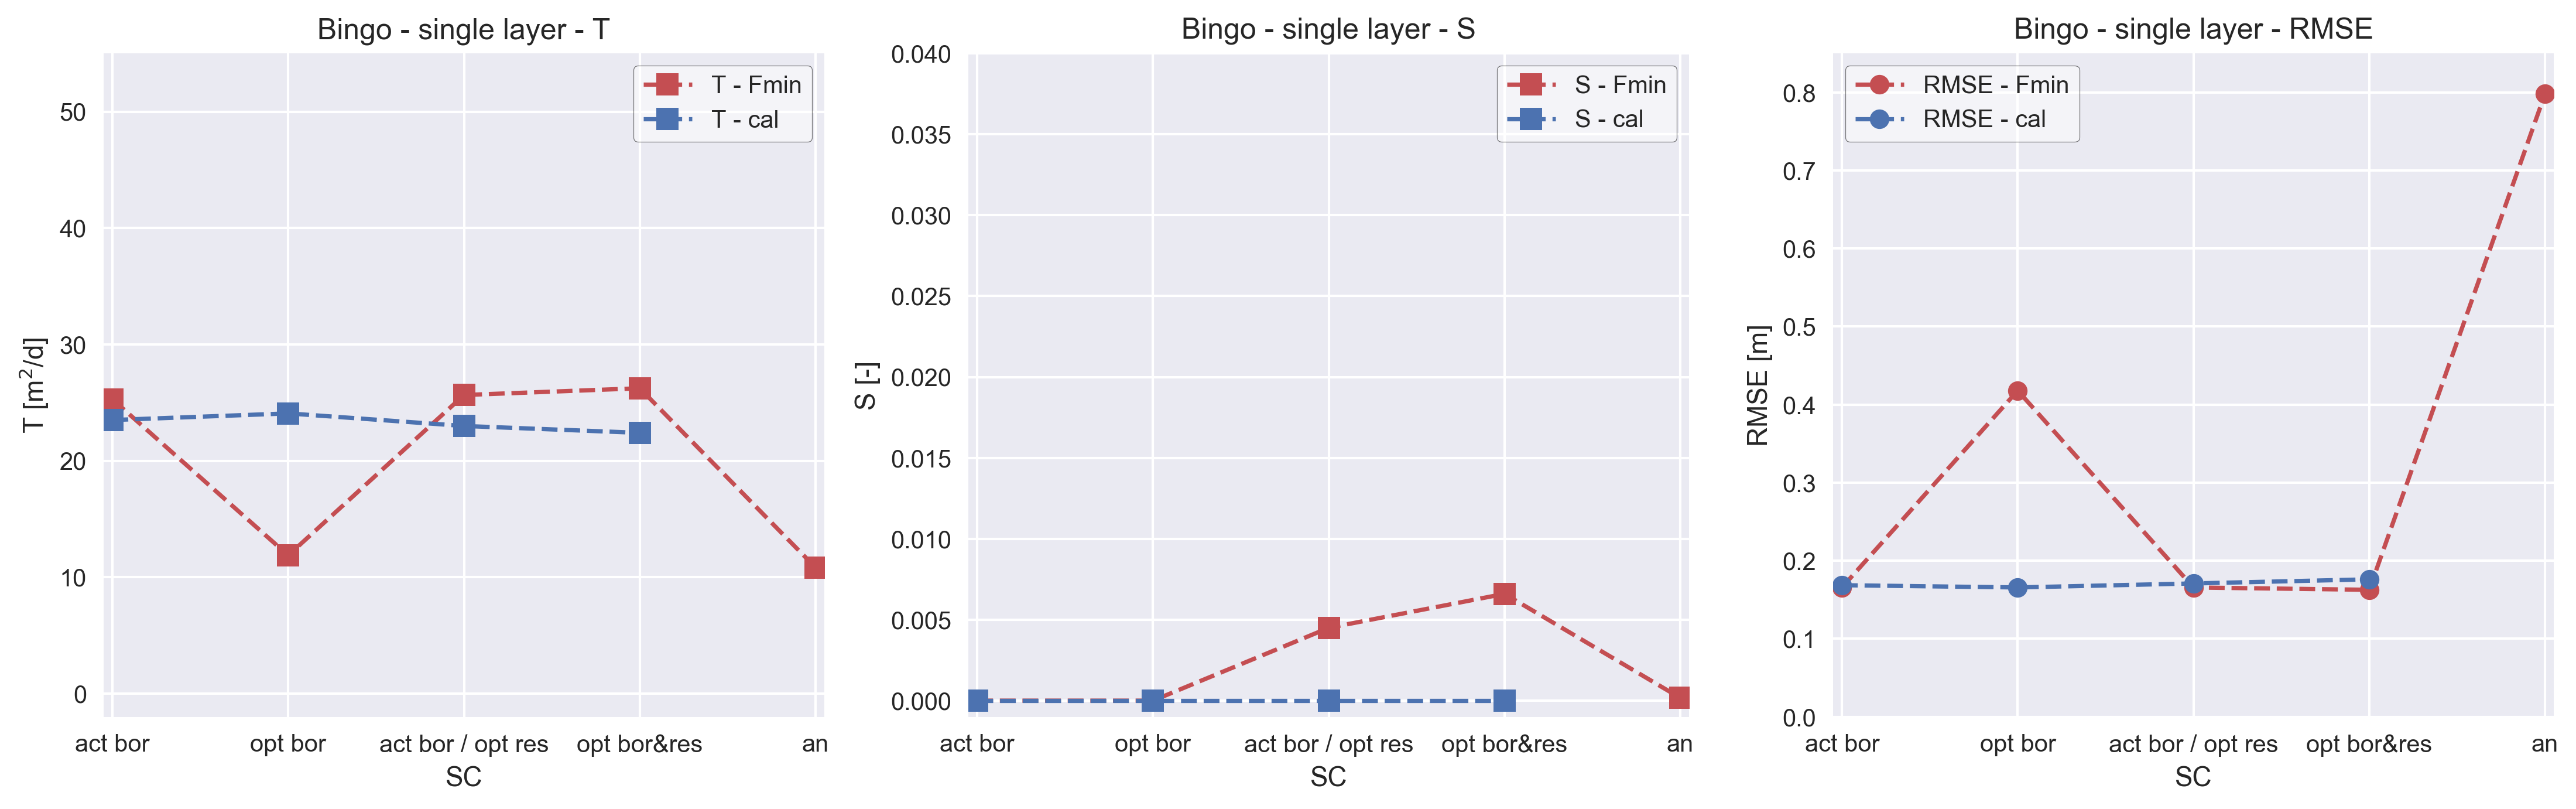
\includegraphics[width=\linewidth]{Bingo_para_results_1lay}
		\captionsetup{justification=centering}		
		\caption{\label{fig:Bingo_para_results_1lay}}
		\end{subfigure}\vfill
	\begin{subfigure}[b]{\linewidth}
		\centering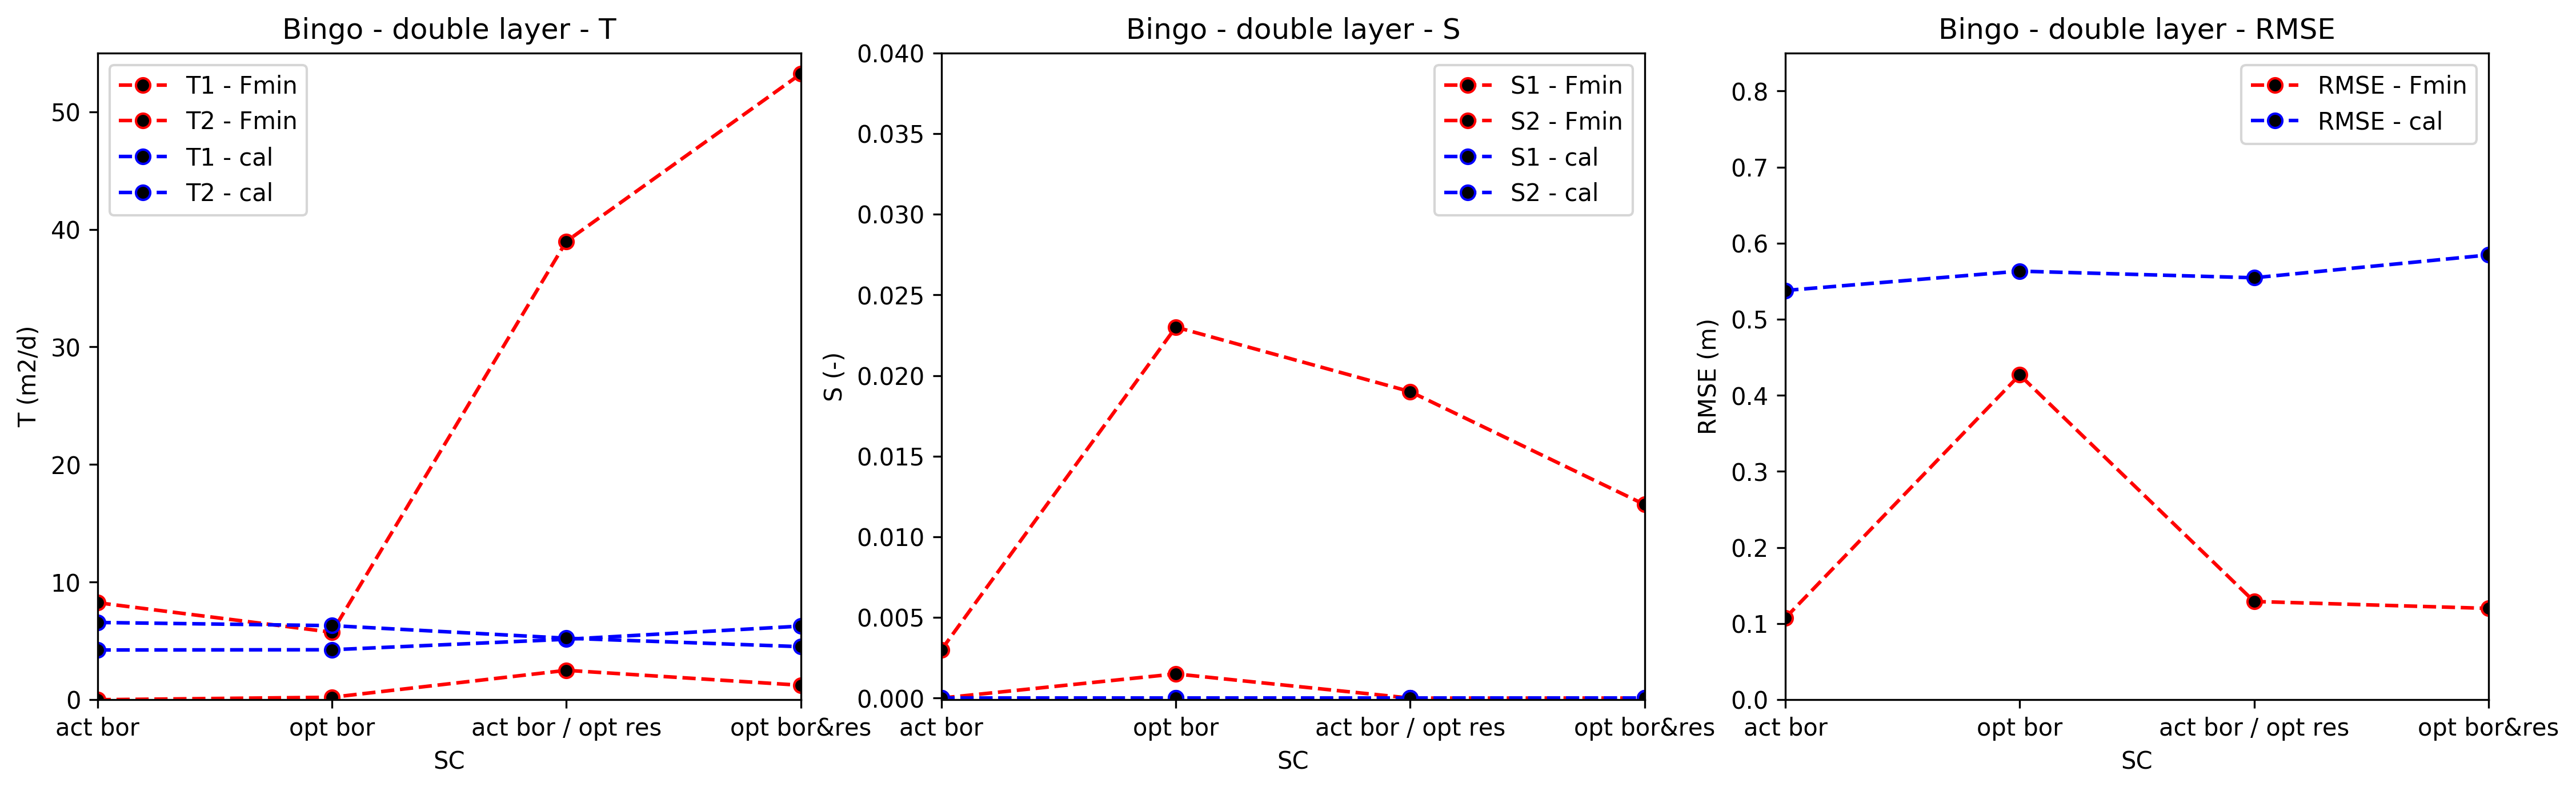
\includegraphics[width=\linewidth]{Bingo_para_results_2lay}
		\captionsetup{justification=centering}		
		\caption{\label{fig:Bingo_para_results_2lay}}
		\end{subfigure}
	\begin{subfigure}[b]{\linewidth}
		\centering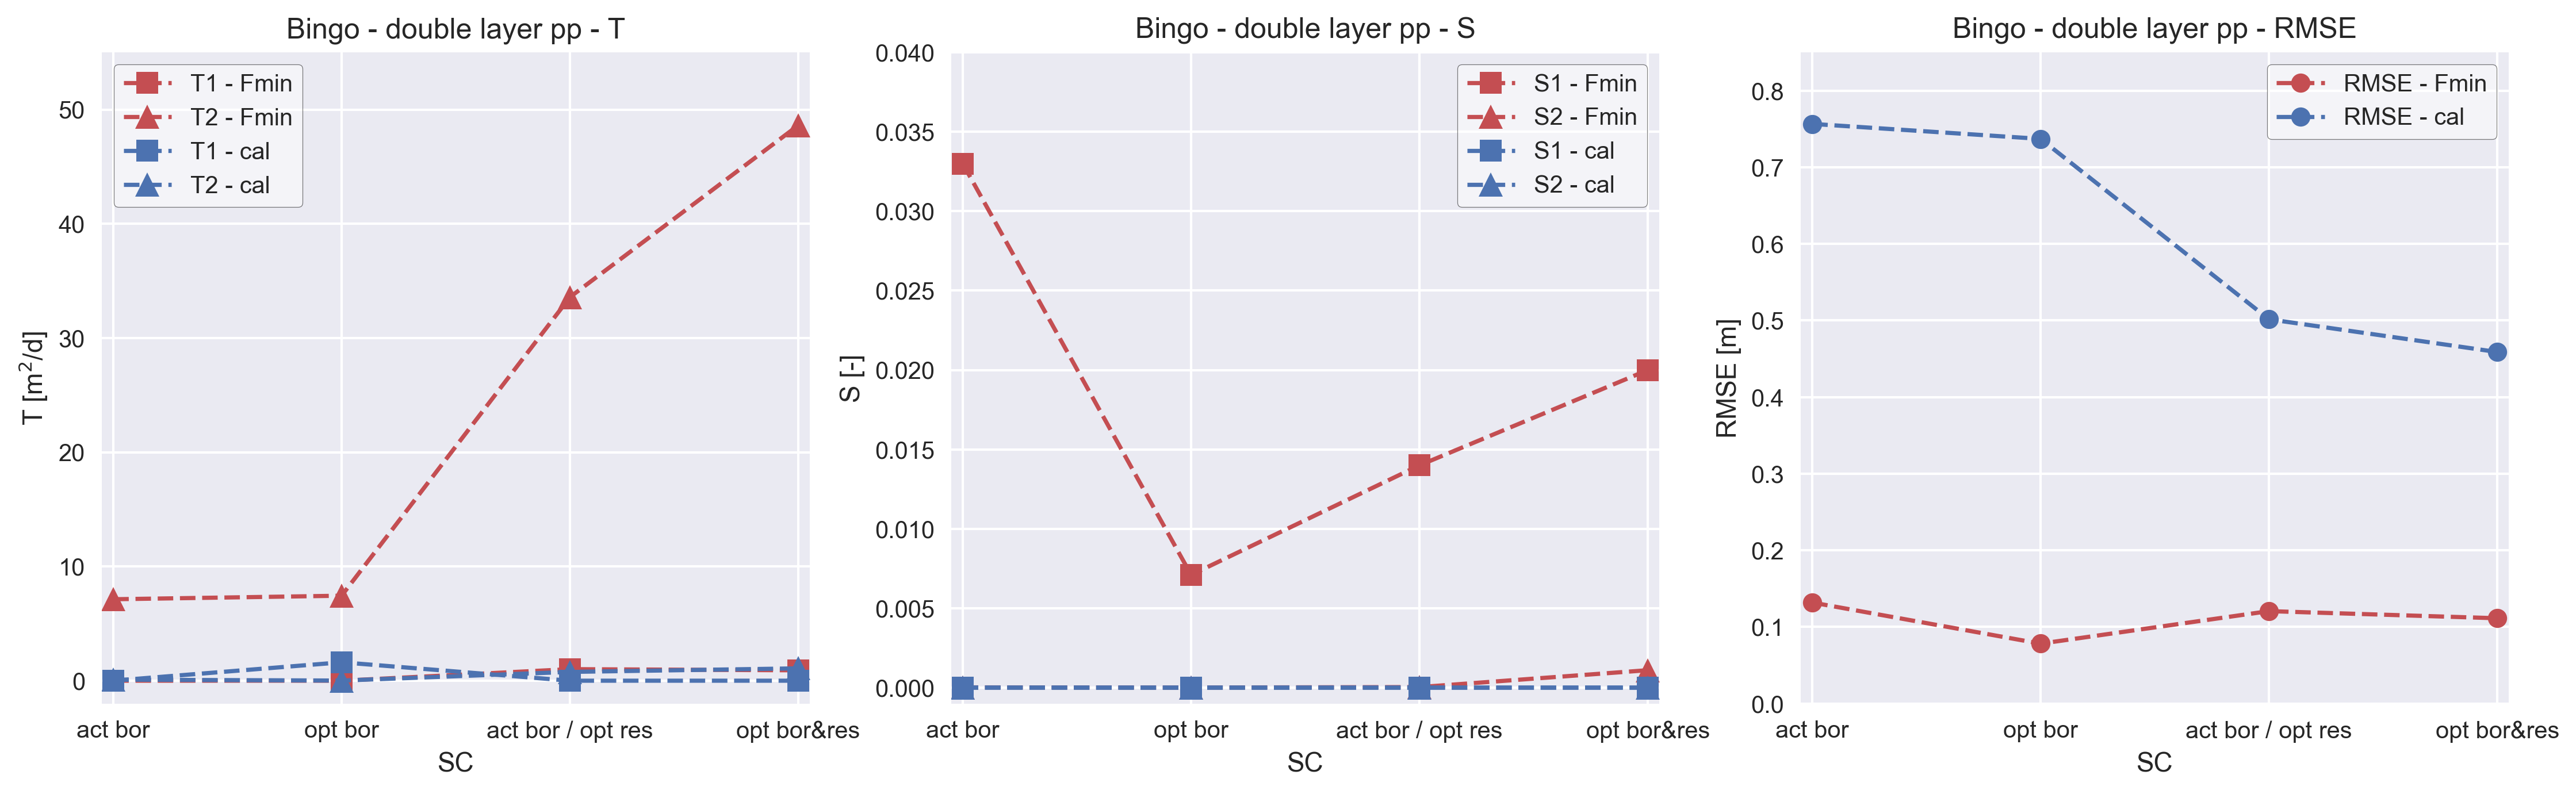
\includegraphics[width=\linewidth]{Bingo_para_results_3lay}
		\captionsetup{justification=centering}		
		\caption{\label{fig:Bingo_para_results_3lay}}
		\end{subfigure}		
	\captionsetup{justification=centering}	
	\caption{Bingo - overview determined (Fmin and Cal) optimal parameter values of (\subref{fig:fig:Bingo_para_results_1lay}) a single layer system, (\subref{fig:fig:Bingo_para_results_2lay}) a double layer system, and (\subref{fig:fig:Bingo_para_results_3lay}) a system with two layers and partial penetration of the well} 
	\label{fig:Bingo_para_results}
\end{figure} 


\clearpage\section{Nungo - overview}
\label{sec:Nungo_overview}
\ bigskip 
Gained fieldwork data at the location Nungo not sufficient for the analysis of geohydrological parameter values.  

\clearpage\section{Nyong Nayili - overview}
\label{sec:Nyong_Nayili_overview}

\begin{figure}[h!]
	\centering
	\begin{subfigure}[b]{0.65\linewidth}
		\centering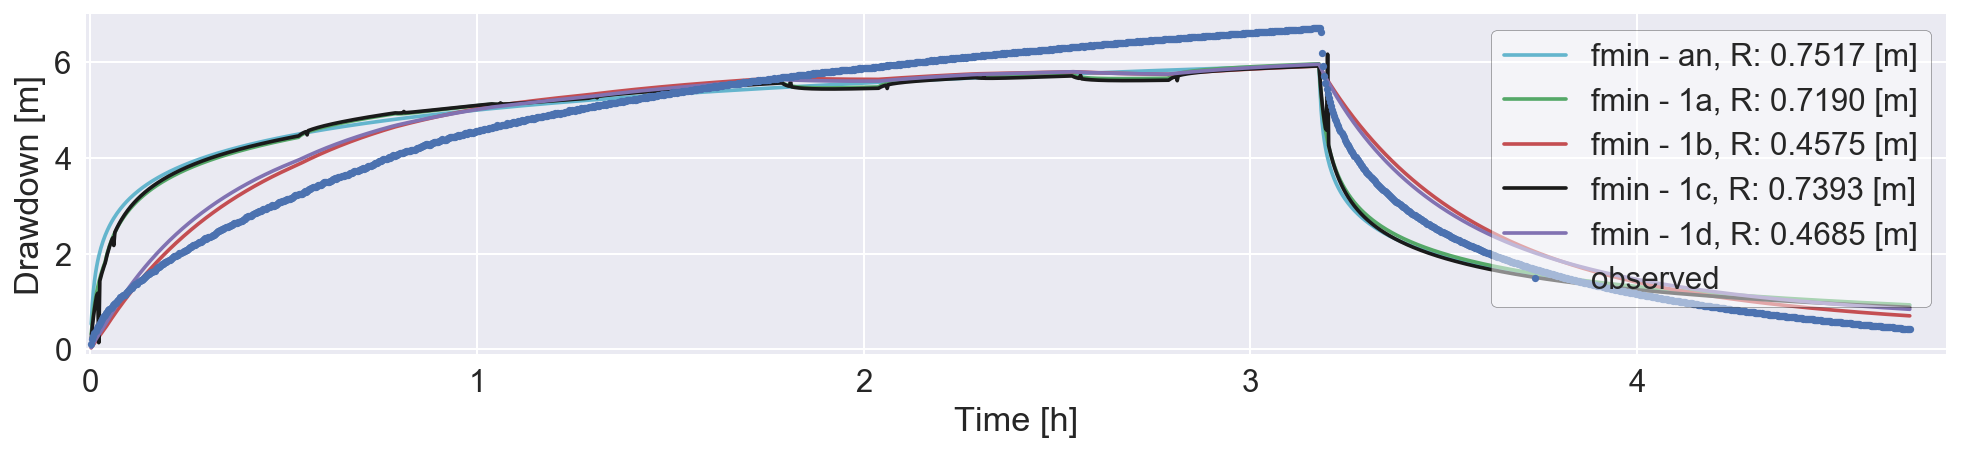
\includegraphics[width=\linewidth]{Nyong_Nayili_1lay_fmin}
		\captionsetup{justification=centering}		
		\caption{\label{fig:Nyong_Nayili_1lay_fmin}}
		\end{subfigure}\vfill
	\begin{subfigure}[b]{0.65\linewidth}
		\centering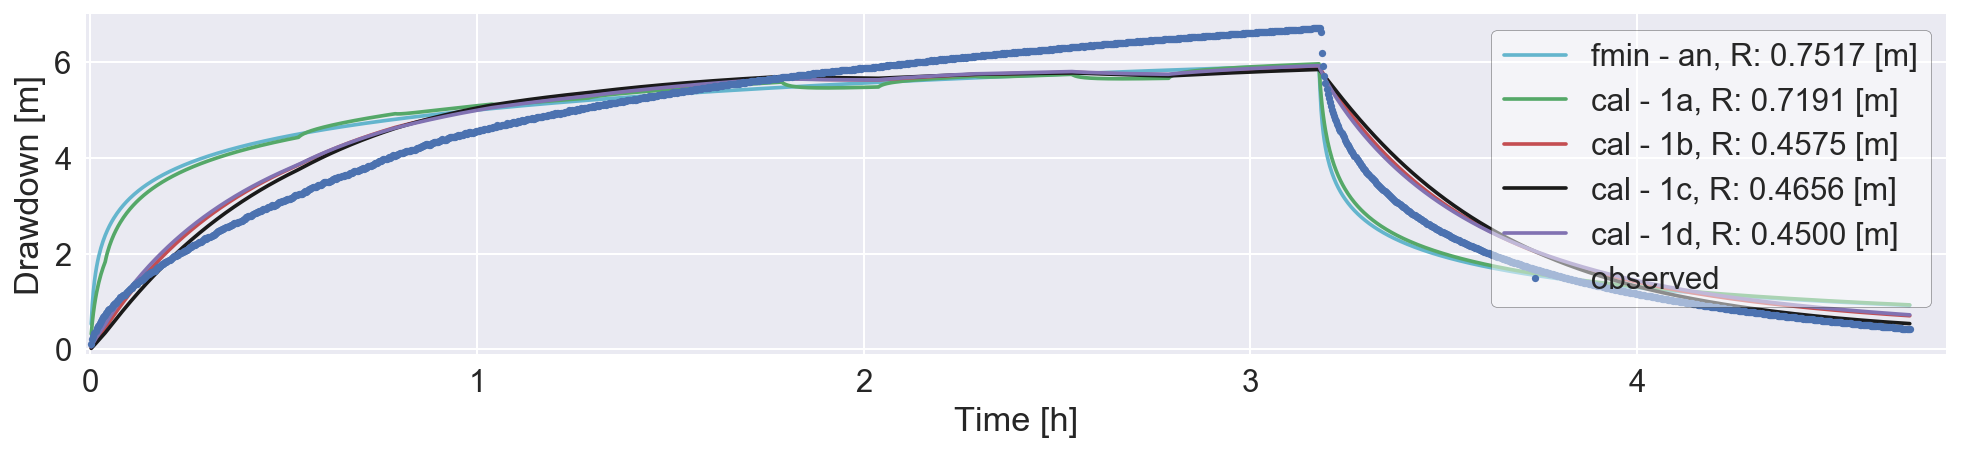
\includegraphics[width=\linewidth]{Nyong_Nayili_1lay_cal}
		\captionsetup{justification=centering}		
		\caption{\label{fig:Nyong_Nayili_1lay_cal}}
		\end{subfigure}
	\captionsetup{justification=centering}	
	\caption{Nyong Nayili single layer fieldwork data analysis by the optimization (\subref{fig:Nyong_Nayili_1lay_fmin}) fmin-RMSE method and (\subref{fig:Nyong_Nayili_1lay_cal}) TTim calibration method} 
	\label{fig:Nyong_Nayili_1lay_analysis}
\end{figure} 

\begin{figure}[h!]
	\centering
	\begin{subfigure}[b]{0.65\linewidth}
		\centering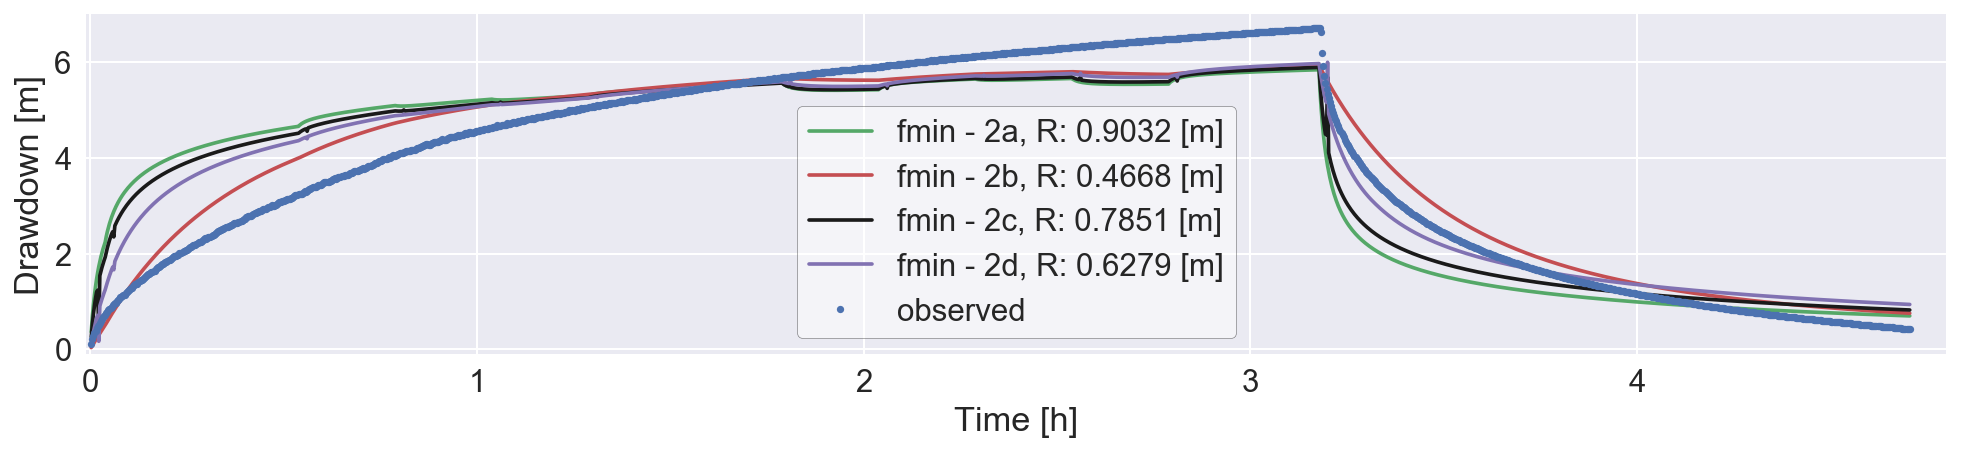
\includegraphics[width=\linewidth]{Nyong_Nayili_2lay_fmin}
		\captionsetup{justification=centering}		
		\caption{\label{fig:Nyong_Nayili_2lay_fmin}}
		\end{subfigure}\vfill
	\begin{subfigure}[b]{0.65\linewidth}
		\centering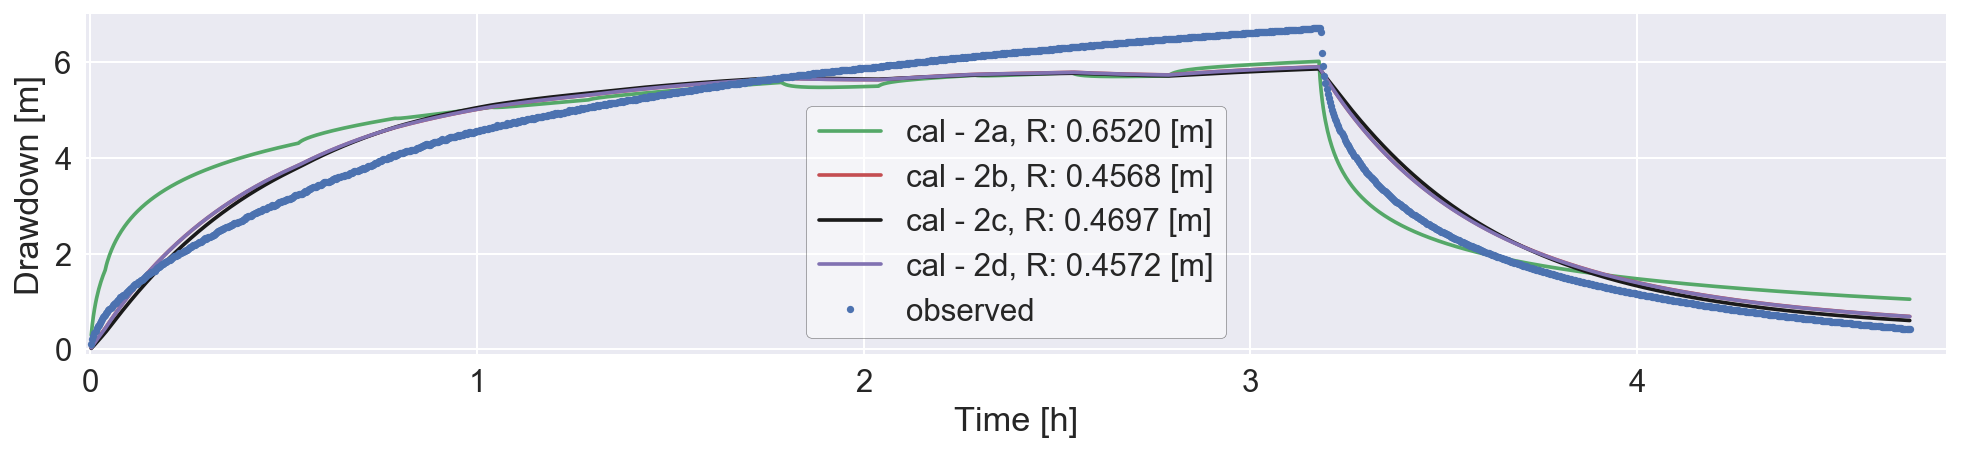
\includegraphics[width=\linewidth]{Nyong_Nayili_2lay_cal}
		\captionsetup{justification=centering}		
		\caption{\label{fig:Nyong_Nayili_2lay_cal}}
		\end{subfigure}
	\captionsetup{justification=centering}	
	\caption{Nyong Nayili double layer fieldwork data analysis by the optimization (\subref{fig:Nyong_Nayili_2lay_fmin}) fmin-RMSE method and (\subref{fig:Nyong_Nayili_2lay_cal}) TTim calibration method} 
	\label{fig:Nyong_Nayili_2lay_analysis}
\end{figure} 

\begin{figure}[h!]
	\centering
	\begin{subfigure}[b]{0.65\linewidth}
		\centering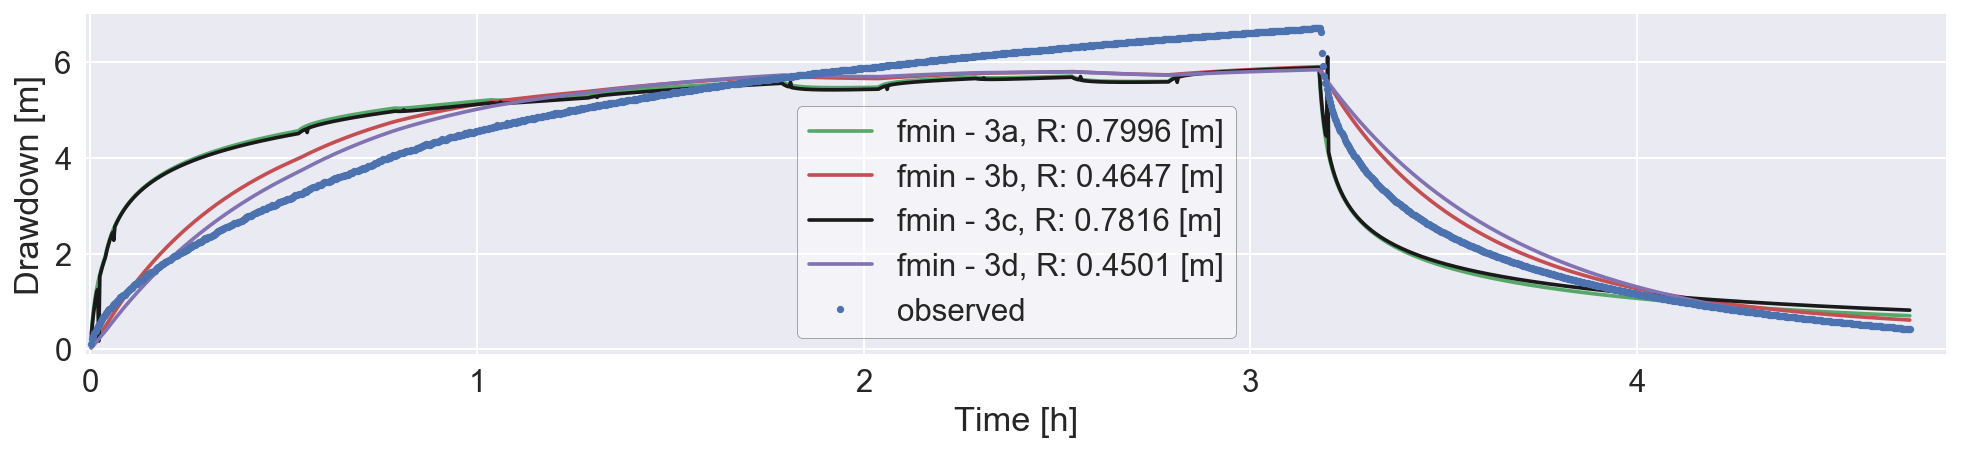
\includegraphics[width=\linewidth]{Nyong_Nayili_3lay_fmin}
		\captionsetup{justification=centering}		
		\caption{\label{fig:Nyong_Nayili_3lay_fmin}}
		\end{subfigure}\vfill
	\begin{subfigure}[b]{0.65\linewidth}
		\centering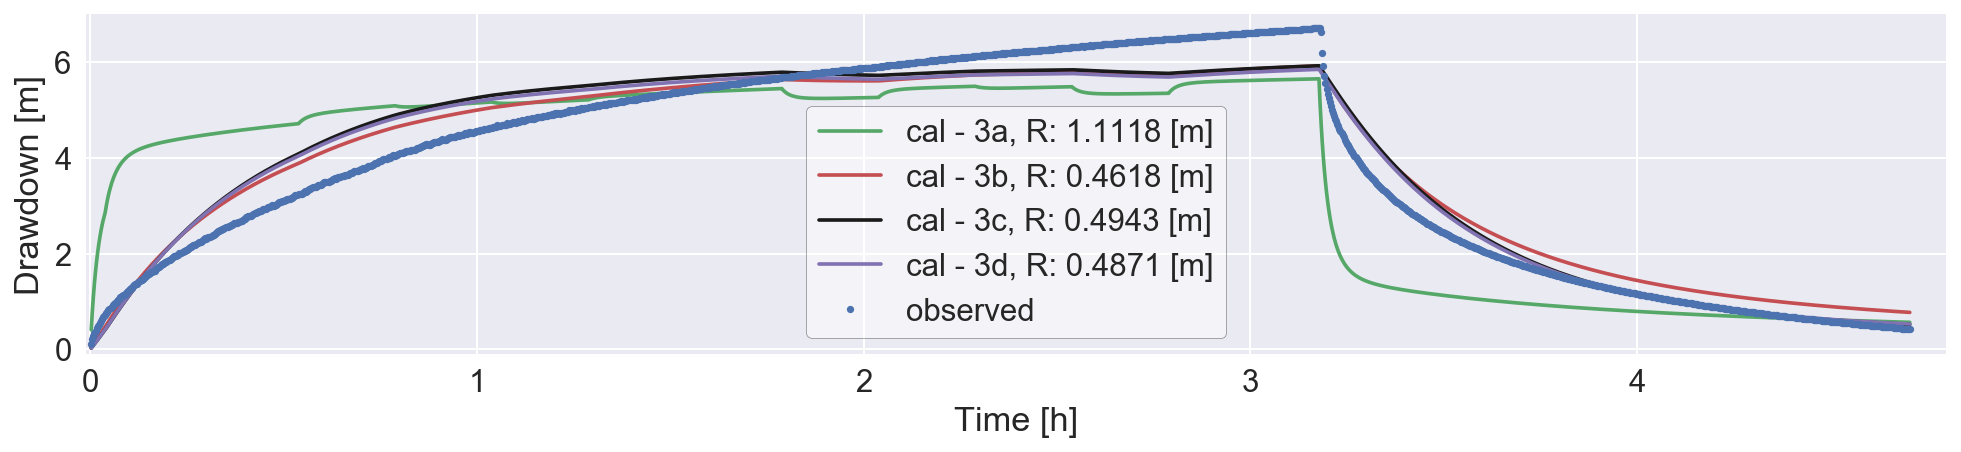
\includegraphics[width=\linewidth]{Nyong_Nayili_3lay_cal}
		\captionsetup{justification=centering}		
		\caption{\label{fig:Nyong_Nayili_3lay_cal}}
		\end{subfigure}
	\captionsetup{justification=centering}	
	\caption{Nyong Nayili partially penetrating double layer fieldwork data analysis by the optimization (\subref{fig:Nyong_Nayili_3lay_fmin}) fmin-RMSE method and (\subref{fig:Nyong_Nayili_3lay_cal}) TTim calibration method} 
	\label{fig:Nyong_Nayili_3lay_analysis}
\end{figure} 

\clearpage

\begin{figure}[h!]
	\centering
	\begin{subfigure}[b]{\linewidth}
		\centering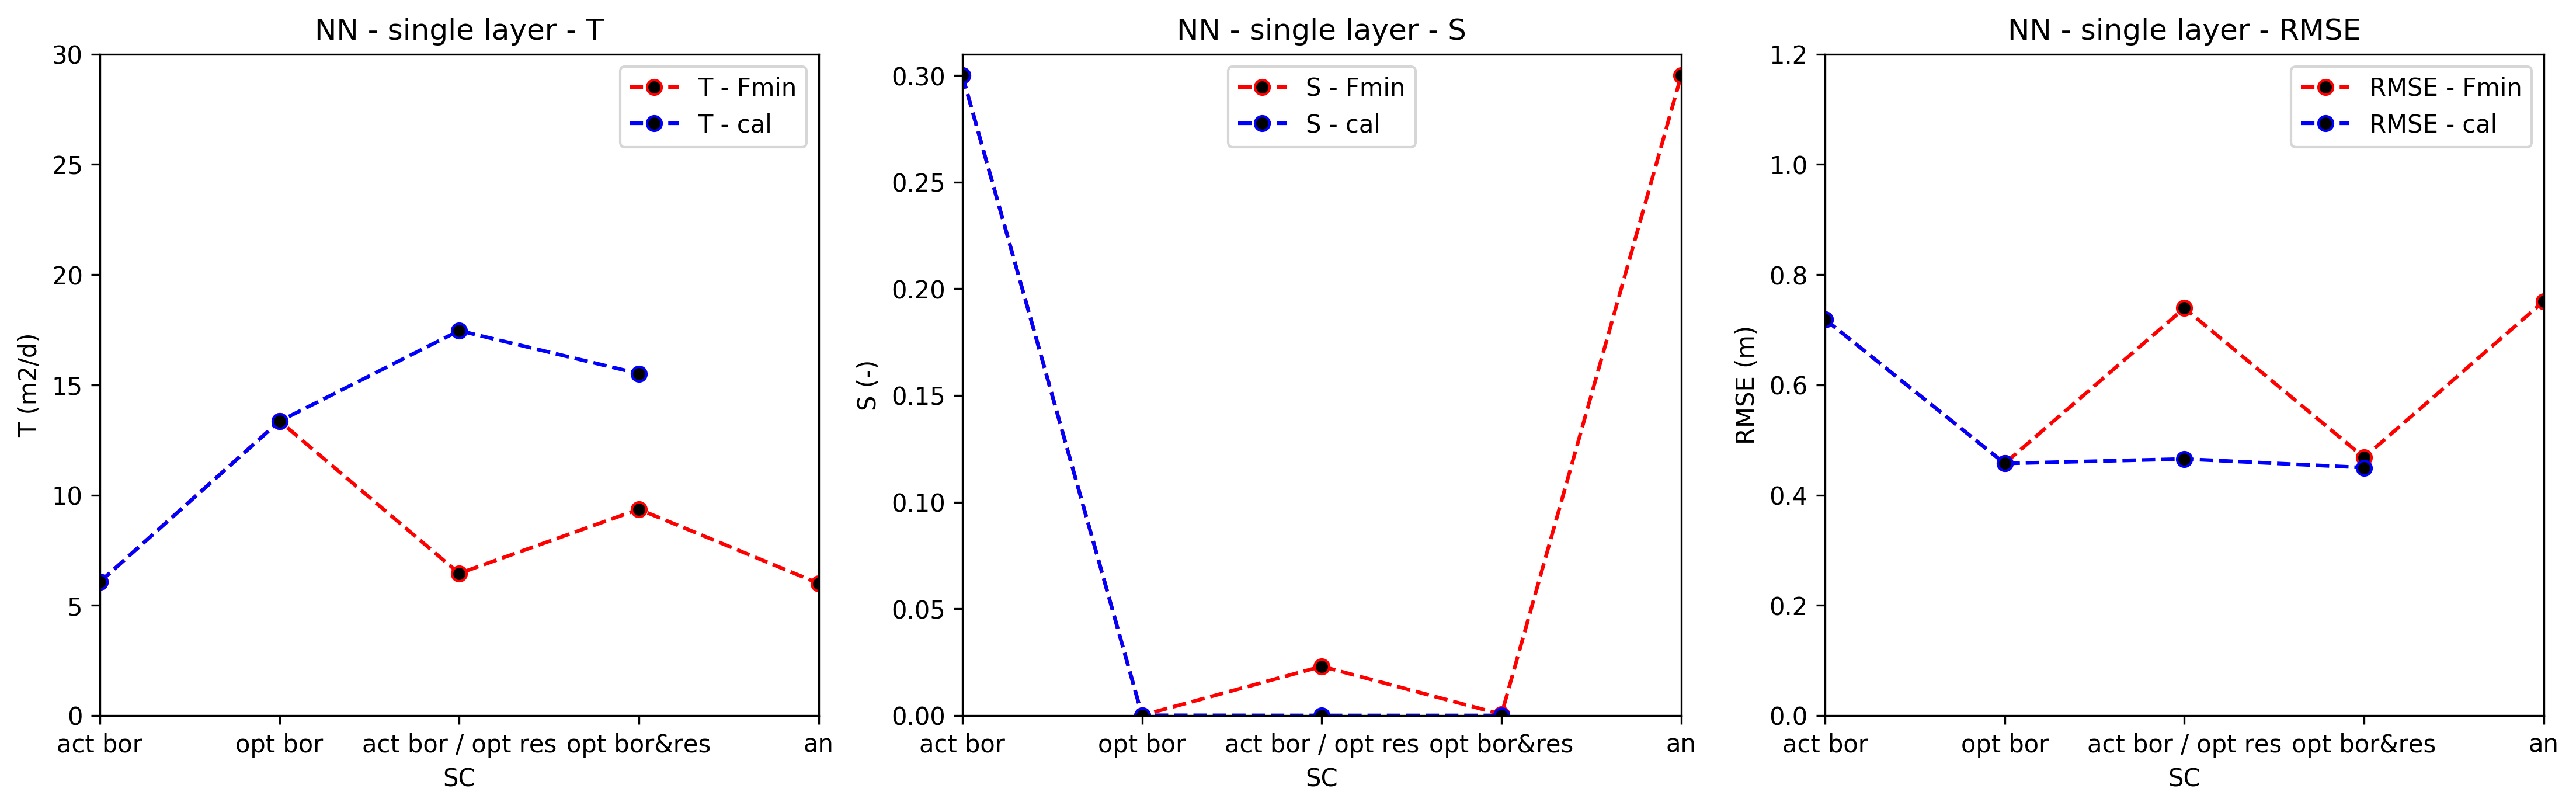
\includegraphics[width=\linewidth]{NN_para_results_1lay}
		\captionsetup{justification=centering}		
		\caption{\label{fig:NN_para_results_1lay}}
		\end{subfigure}\vfill
	\begin{subfigure}[b]{\linewidth}
		\centering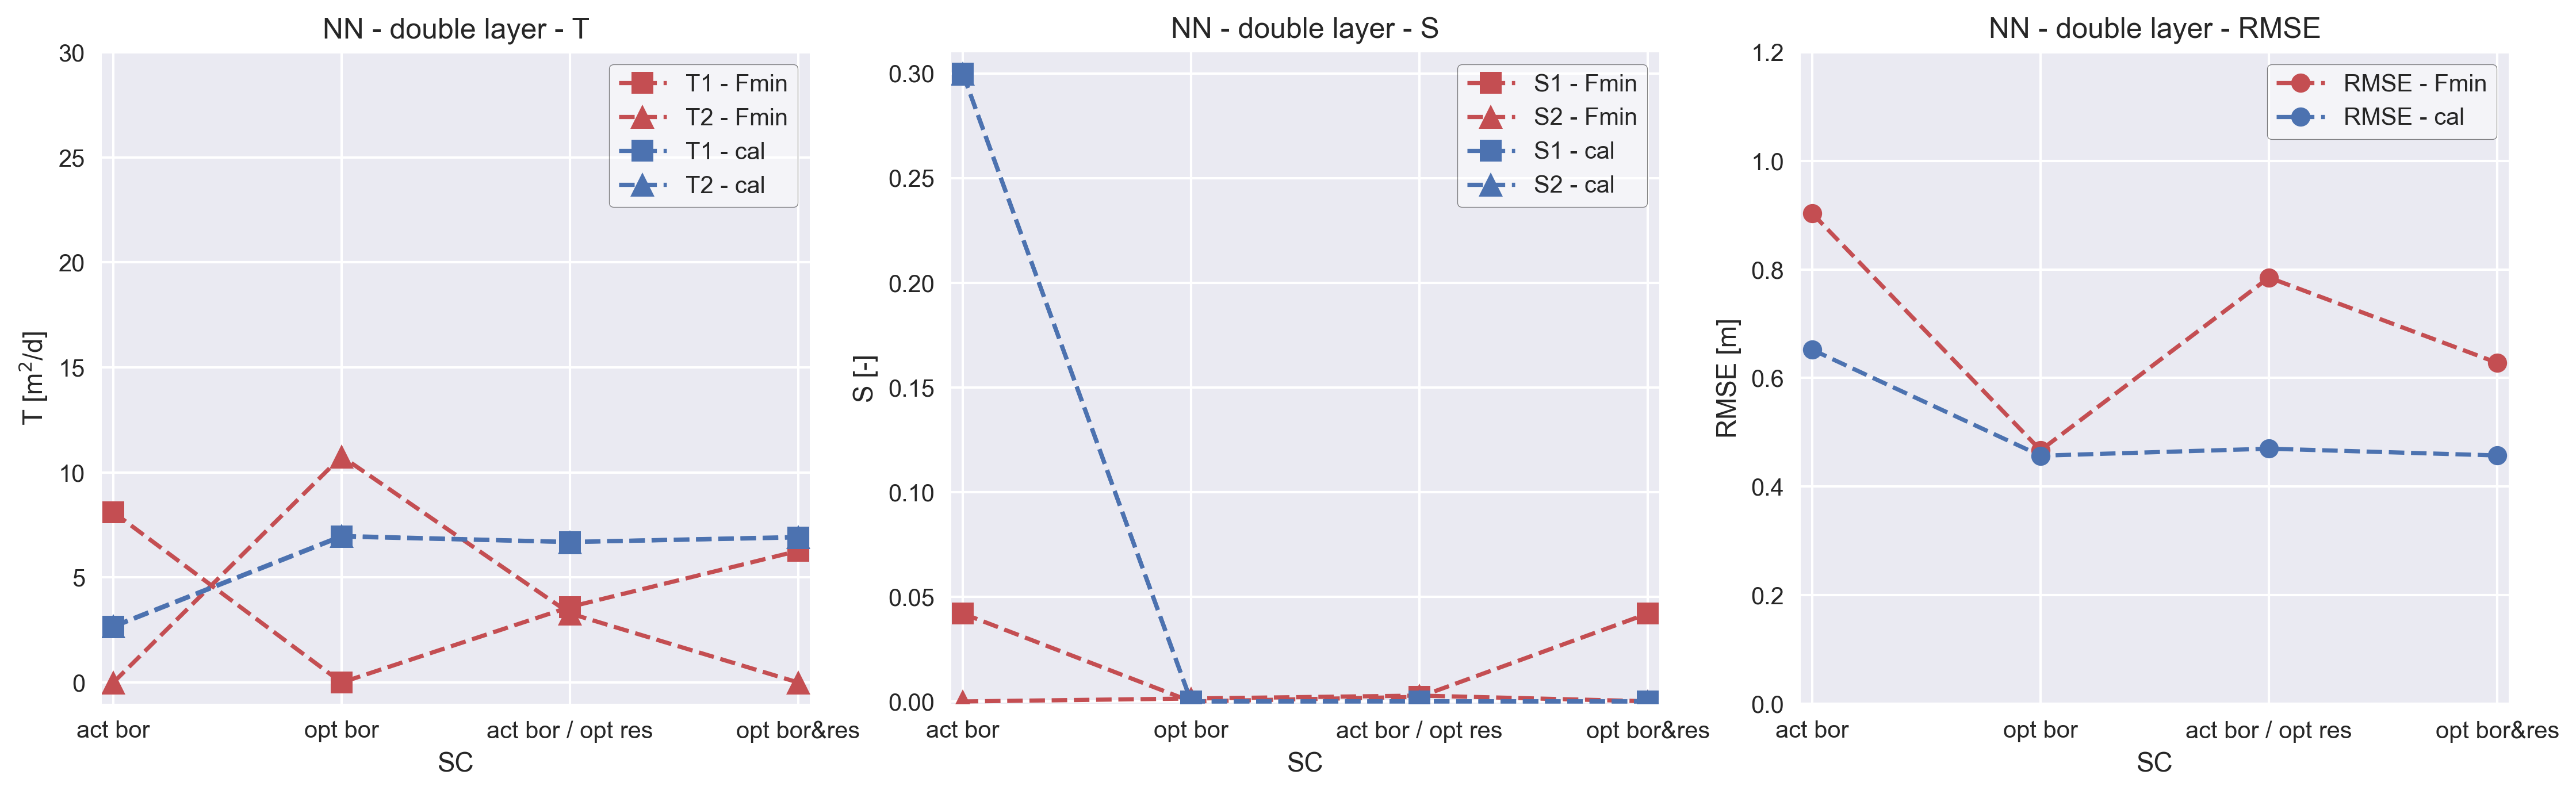
\includegraphics[width=\linewidth]{NN_para_results_2lay}
		\captionsetup{justification=centering}		
		\caption{\label{fig:NN_para_results_2lay}}
		\end{subfigure}
	\begin{subfigure}[b]{\linewidth}
		\centering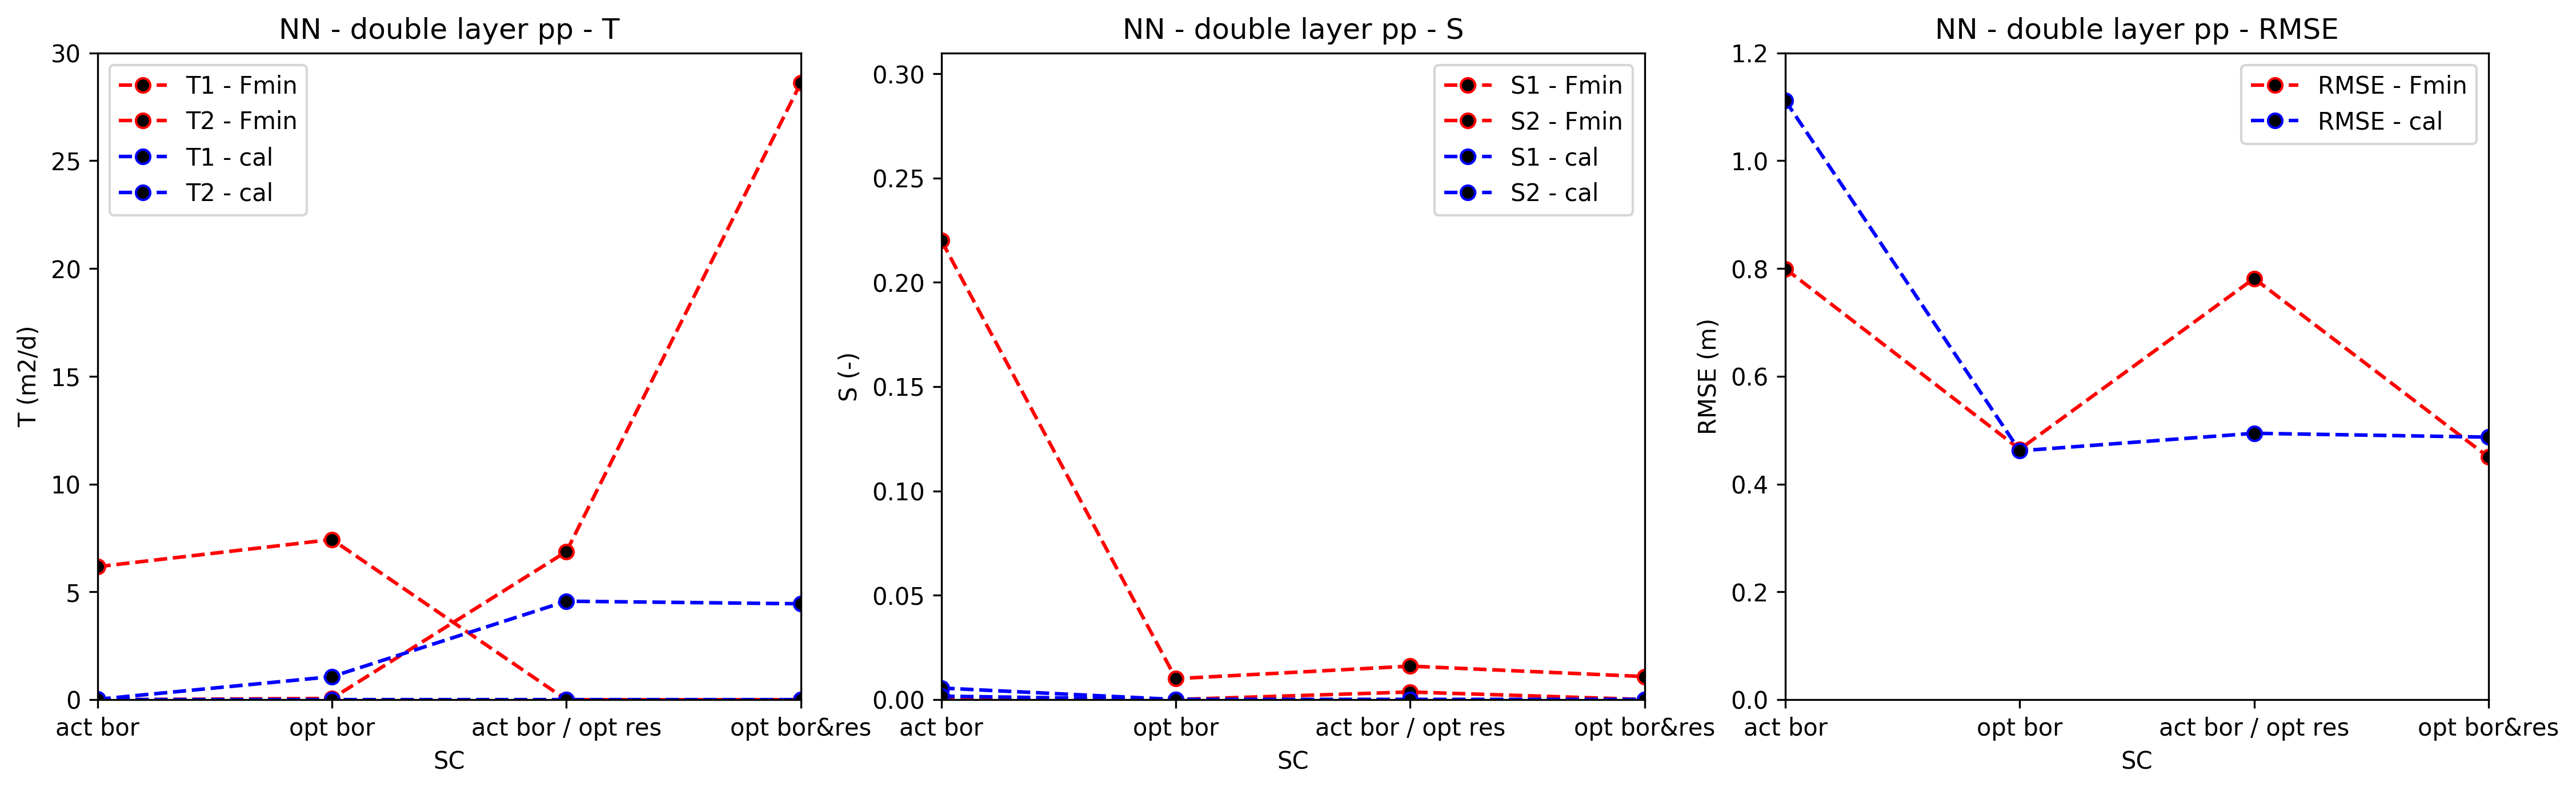
\includegraphics[width=\linewidth]{NN_para_results_3lay}
		\captionsetup{justification=centering}		
		\caption{\label{fig:NN_para_results_3lay}}
		\end{subfigure}		
	\captionsetup{justification=centering}	
	\caption{Nyong Nayili - overview determined (Fmin and Cal) optimal parameter values of (\subref{fig:fig:NN_para_results_1lay}) a single layer system, (\subref{fig:fig:NN_para_results_2lay}) a double layer system, and (\subref{fig:fig:NN_para_results_3lay}) a system with two layers and partial penetration of the well} 
	\label{fig:NN_para_results}
\end{figure} 


\clearpage\section{Janga (1/2) - overview}
\label{sec:Janga1_overview}

\begin{figure}[h!]
	\centering
	\begin{subfigure}[b]{0.65\linewidth}
		\centering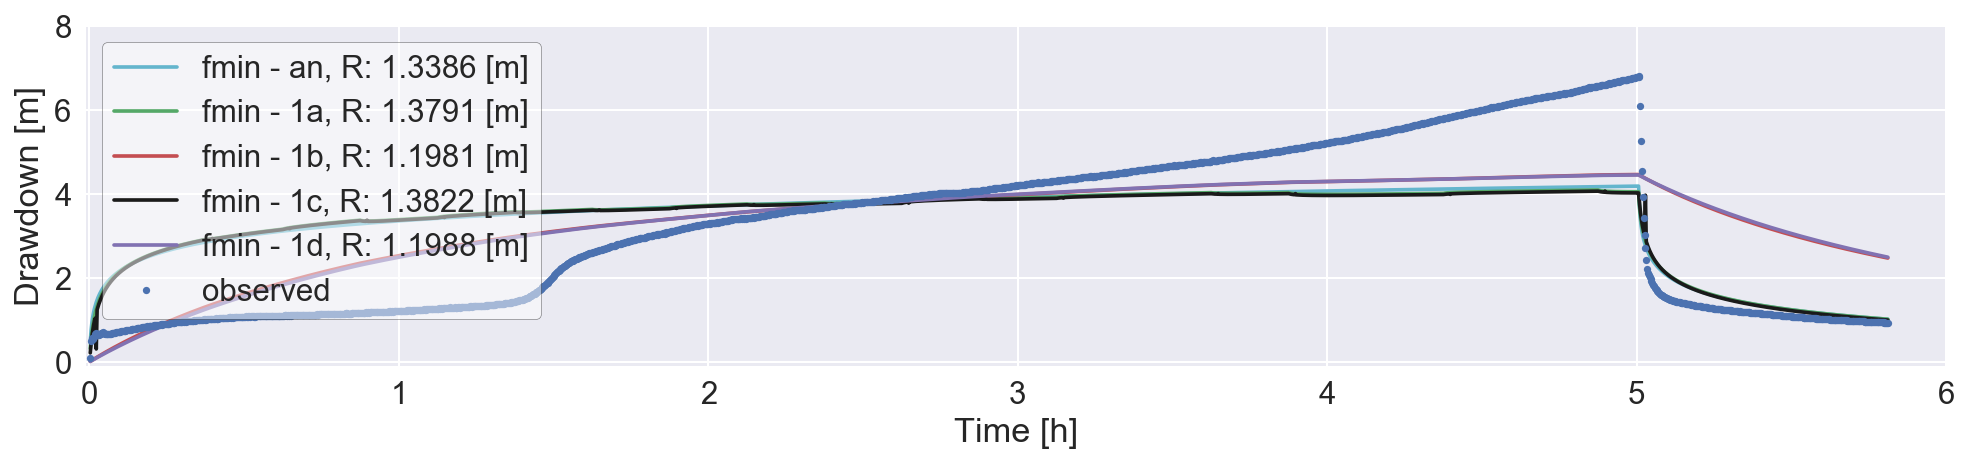
\includegraphics[width=\linewidth]{Janga1_1lay_fmin}
		\captionsetup{justification=centering}		
		\caption{\label{fig:Janga1_1lay_fmin}}
		\end{subfigure}\vfill
	\begin{subfigure}[b]{0.65\linewidth}
		\centering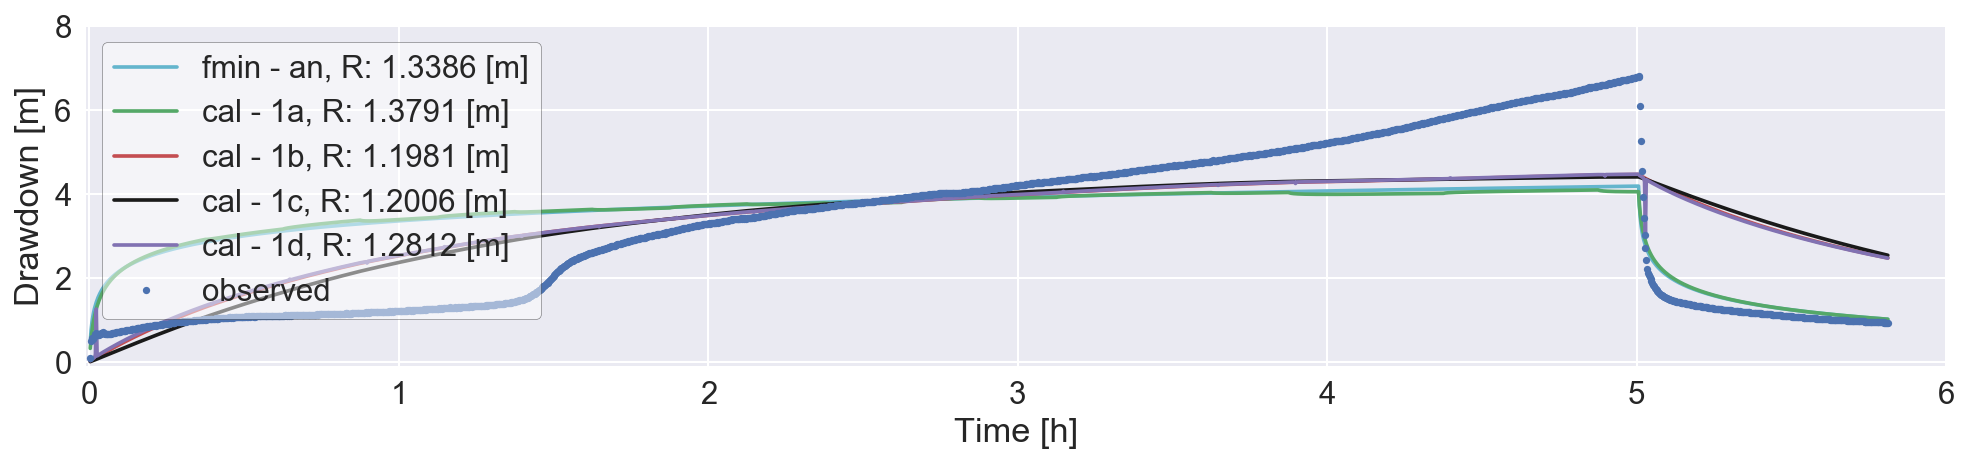
\includegraphics[width=\linewidth]{Janga1_1lay_cal}
		\captionsetup{justification=centering}		
		\caption{\label{fig:Janga1_1lay_cal}}
		\end{subfigure}
	\captionsetup{justification=centering}	
	\caption{Janga first attempt single layer fieldwork data analysis by the optimization (\subref{fig:Janga1_1lay_fmin}) fmin-RMSE method and (\subref{fig:Janga1_1lay_cal}) TTim calibration method} 
	\label{fig:Janga1_1lay_analysis}
\end{figure} 

\begin{figure}[h!]
	\centering
	\begin{subfigure}[b]{0.65\linewidth}
		\centering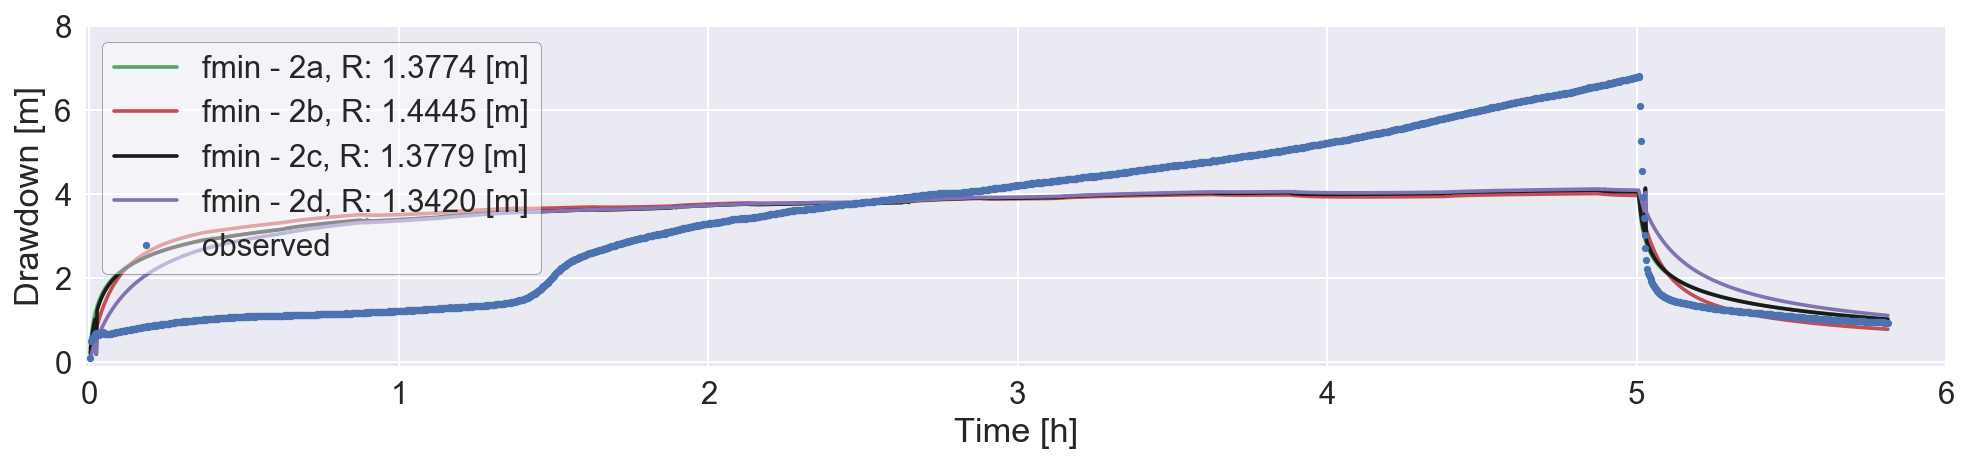
\includegraphics[width=\linewidth]{Janga1_2lay_fmin}
		\captionsetup{justification=centering}		
		\caption{\label{fig:Janga1_2lay_fmin}}
		\end{subfigure}\vfill
	\begin{subfigure}[b]{0.65\linewidth}
		\centering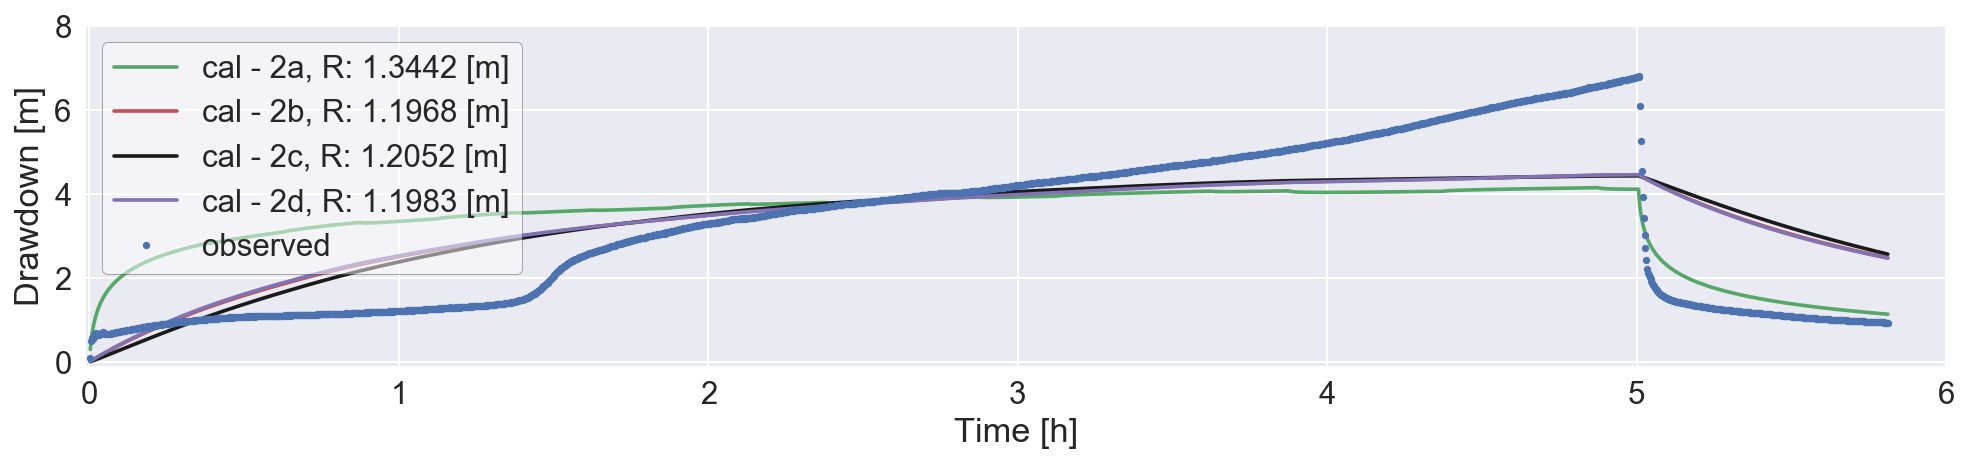
\includegraphics[width=\linewidth]{Janga1_2lay_cal}
		\captionsetup{justification=centering}		
		\caption{\label{fig:Janga1_2lay_cal}}
		\end{subfigure}
	\captionsetup{justification=centering}	
	\caption{Janga first attempt double layer fieldwork data analysis by the optimization (\subref{fig:Janga1_2lay_fmin}) fmin-RMSE method and (\subref{fig:Janga1_2lay_cal}) TTim calibration method} 
	\label{fig:Janga1_2lay_analysis}
\end{figure} 

\begin{figure}[h!]
	\centering
	\begin{subfigure}[b]{0.65\linewidth}
		\centering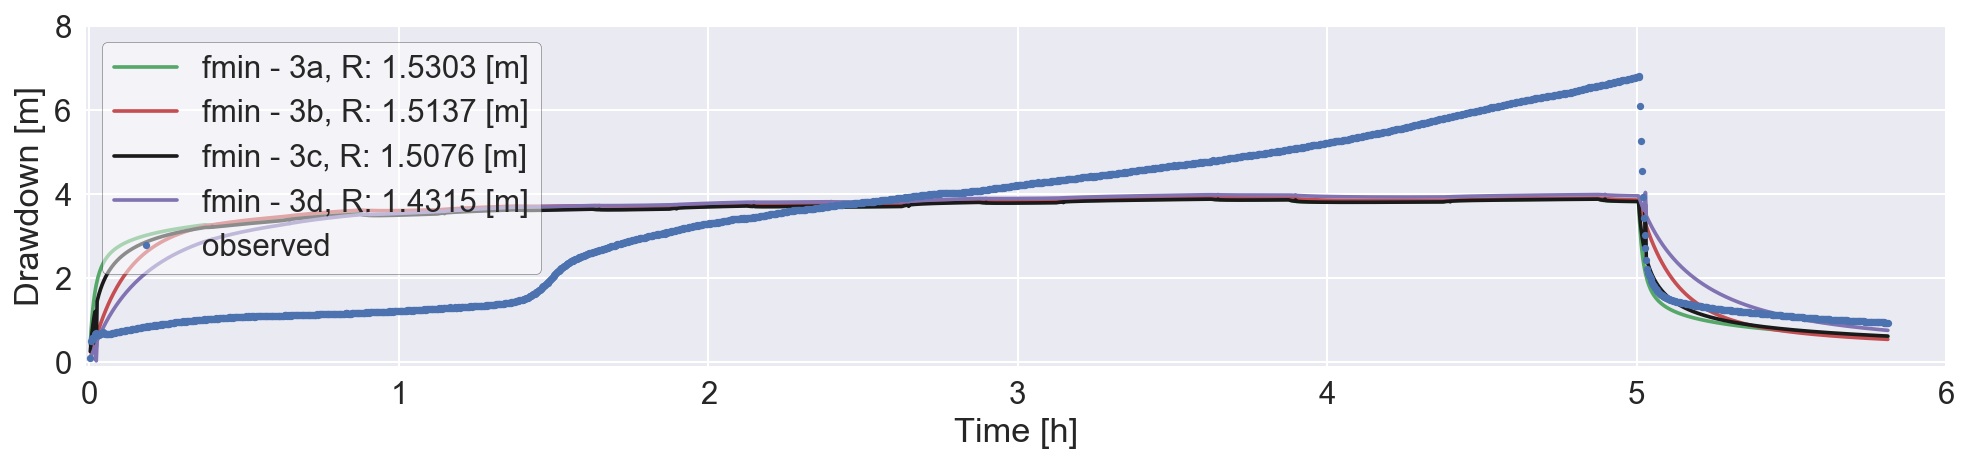
\includegraphics[width=\linewidth]{Janga1_3lay_fmin}
		\captionsetup{justification=centering}		
		\caption{\label{fig:Janga1_3lay_fmin}}
		\end{subfigure}\vfill
	\begin{subfigure}[b]{0.65\linewidth}
		\centering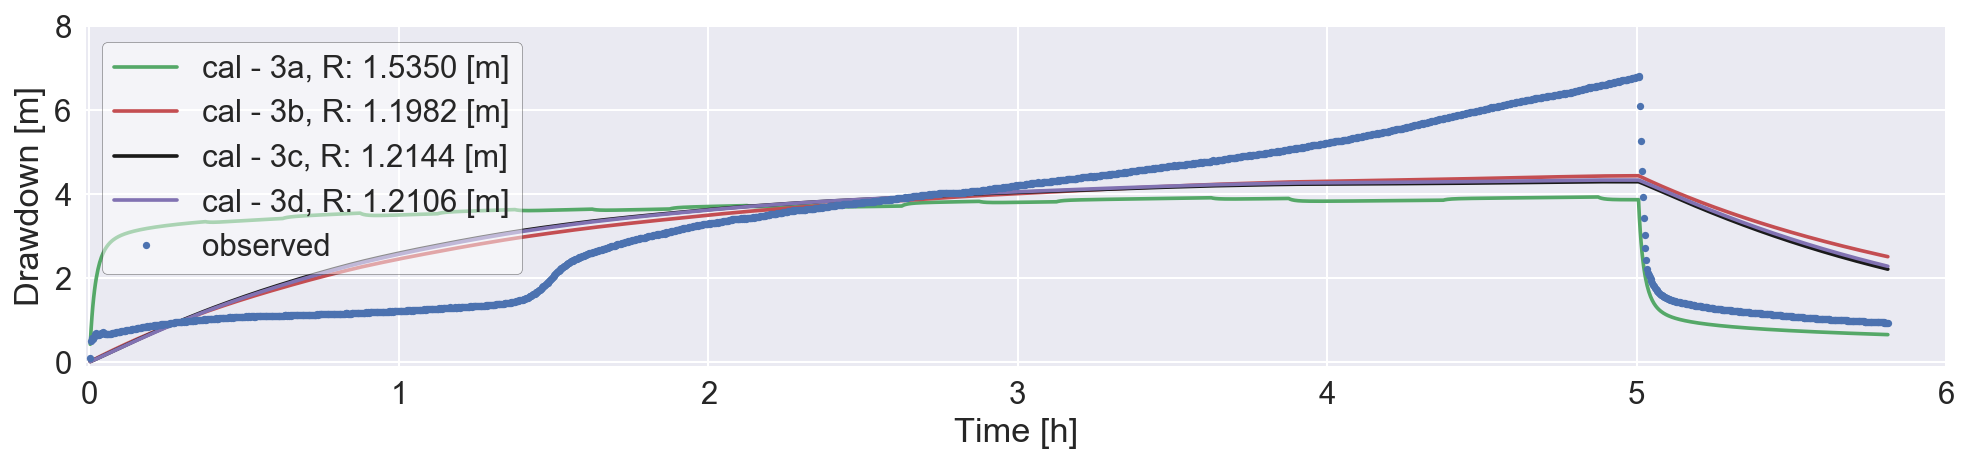
\includegraphics[width=\linewidth]{Janga1_3lay_cal}
		\captionsetup{justification=centering}		
		\caption{\label{fig:Janga1_3lay_cal}}
		\end{subfigure}
	\captionsetup{justification=centering}	
	\caption{Janga first attempt partially penetrating double layer fieldwork data analysis by the optimization (\subref{fig:Janga1_3lay_fmin}) fmin-RMSE method and (\subref{fig:Janga1_3lay_cal}) TTim calibration method} 
	\label{fig:Janga1_3lay_analysis}
\end{figure} 

\clearpage

\begin{figure}[h!]
	\centering
	\begin{subfigure}[b]{\linewidth}
		\centering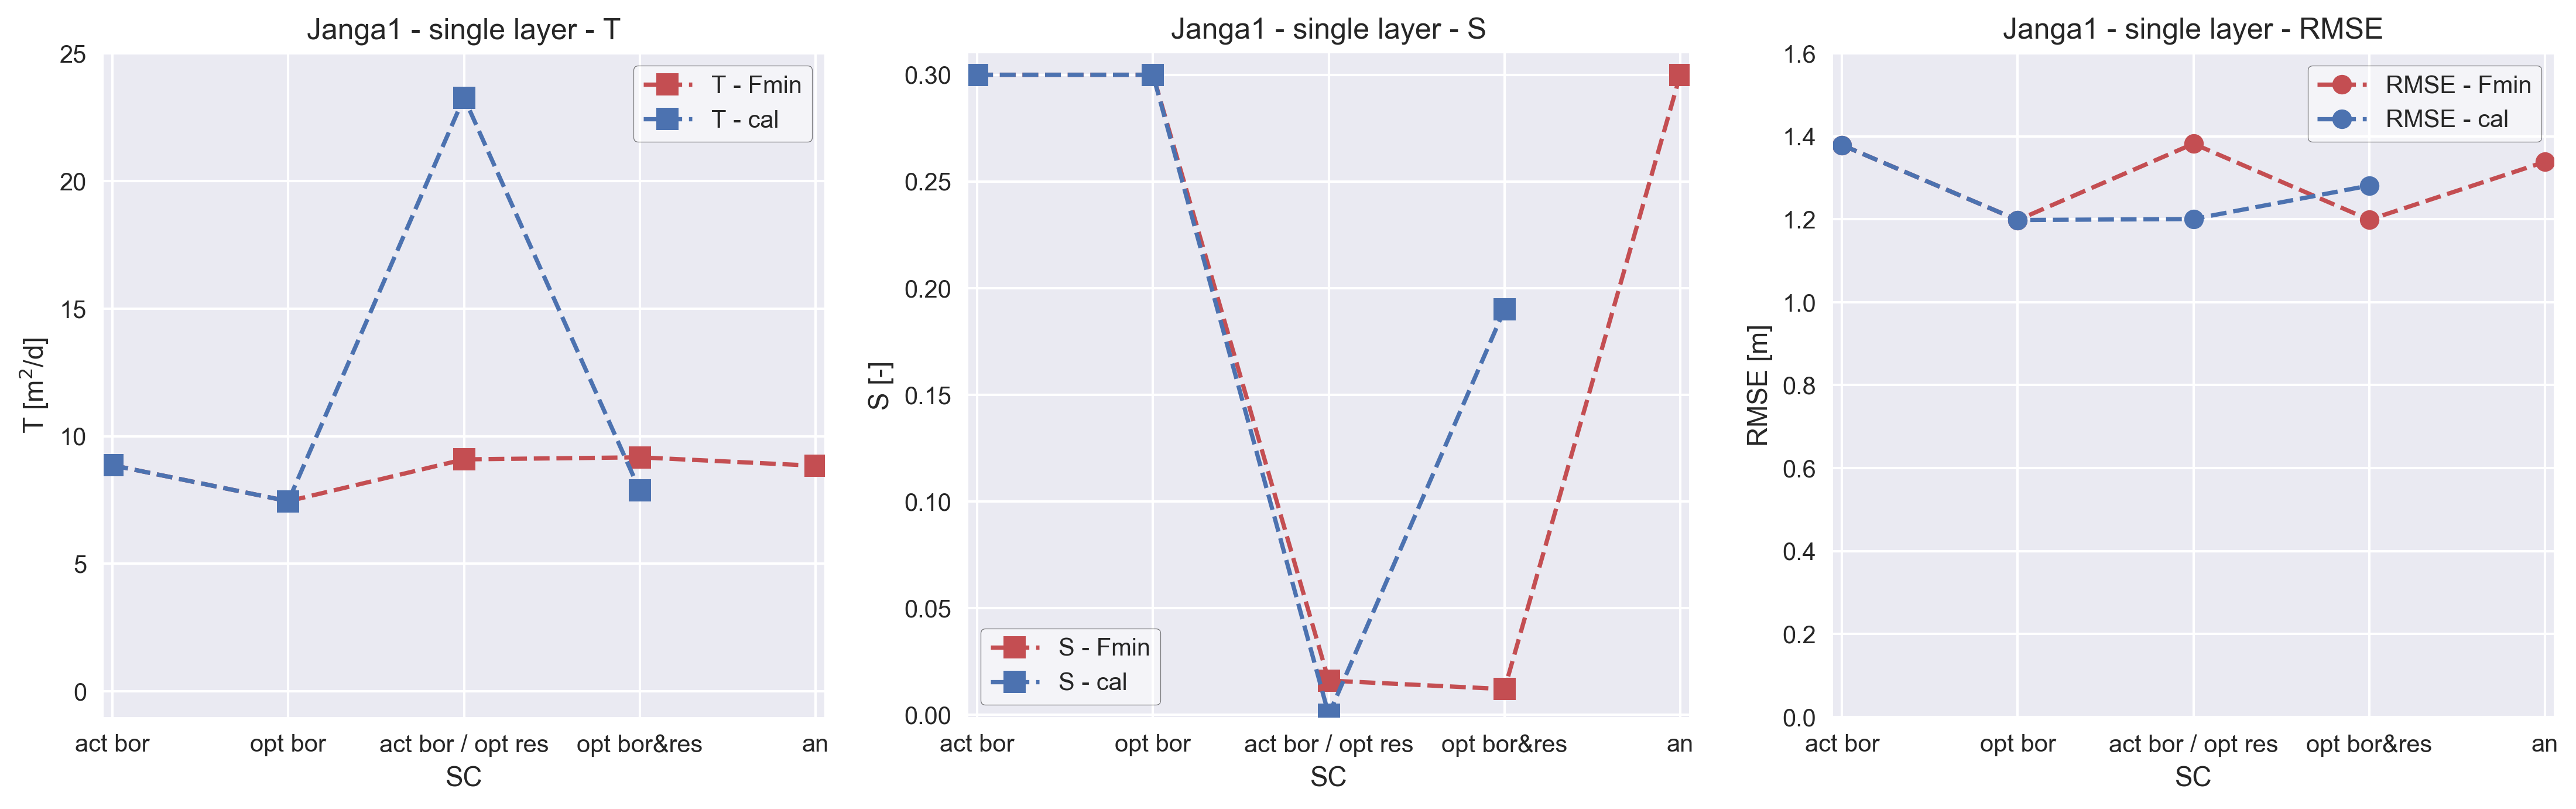
\includegraphics[width=\linewidth]{J1_para_results_1lay}
		\captionsetup{justification=centering}		
		\caption{\label{fig:J1_para_results_1lay}}
		\end{subfigure}\vfill
	\begin{subfigure}[b]{\linewidth}
		\centering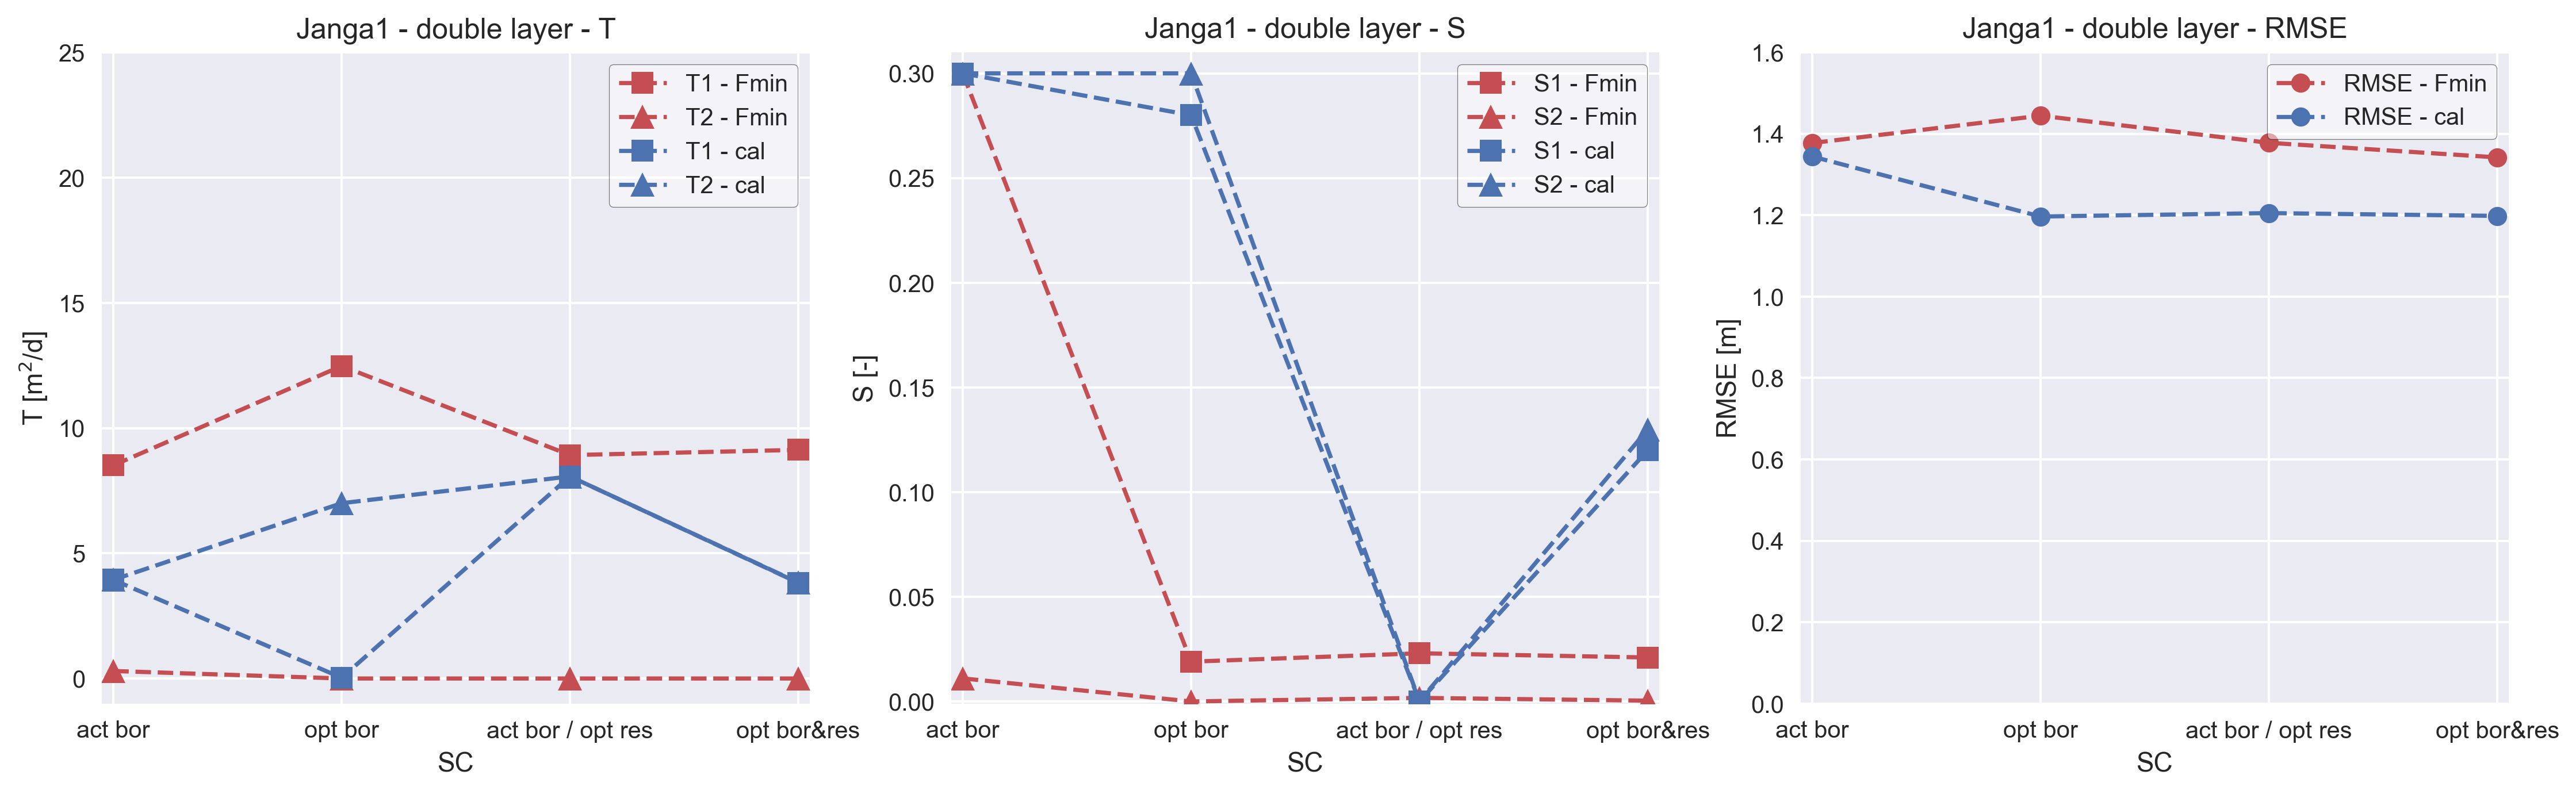
\includegraphics[width=\linewidth]{J1_para_results_2lay}
		\captionsetup{justification=centering}		
		\caption{\label{fig:J1_para_results_2lay}}
		\end{subfigure}
	\begin{subfigure}[b]{\linewidth}
		\centering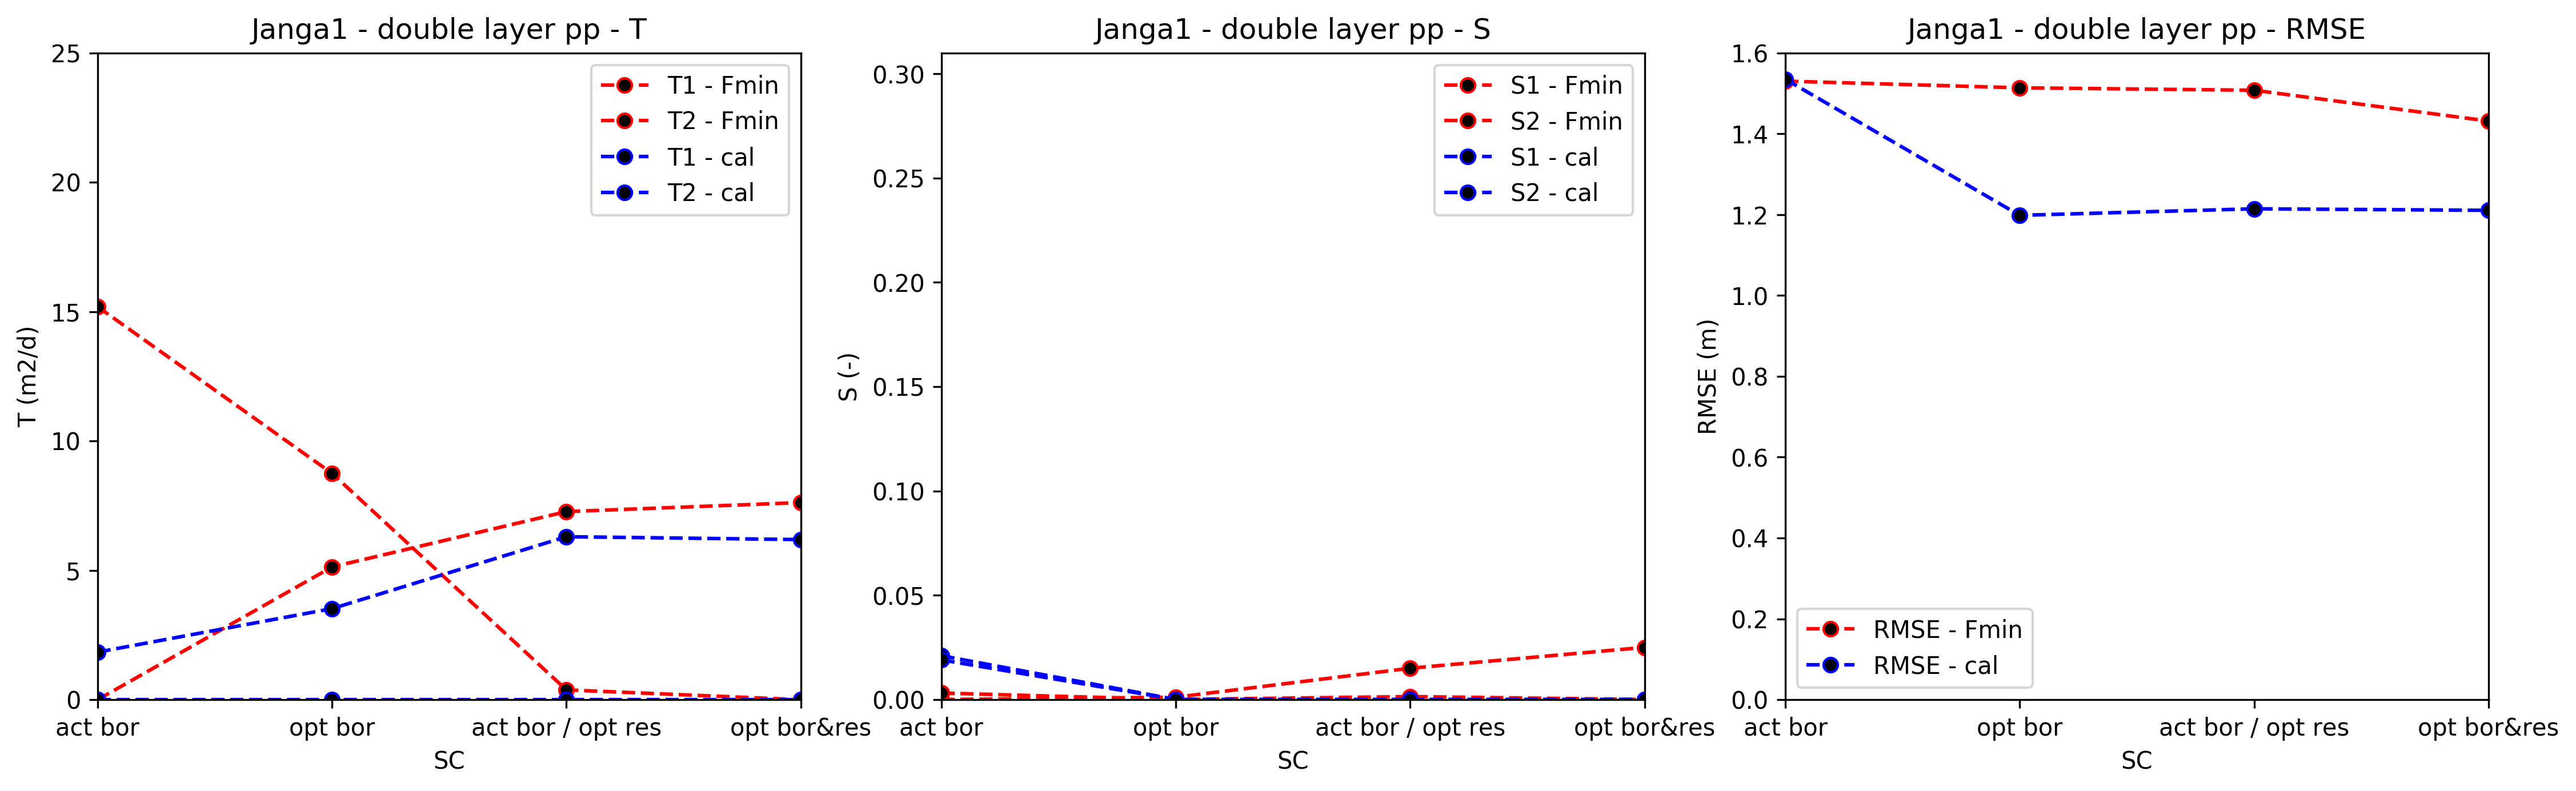
\includegraphics[width=\linewidth]{J1_para_results_3lay}
		\captionsetup{justification=centering}		
		\caption{\label{fig:J1_para_results_3lay}}
		\end{subfigure}		
	\captionsetup{justification=centering}	
	\caption{Janga first attempt - overview determined (Fmin and Cal) optimal parameter values of (\subref{fig:fig:J1_para_results_1lay}) a single layer system, (\subref{fig:fig:J1_para_results_2lay}) a double layer system, and (\subref{fig:fig:J1_para_results_3lay}) a system with two layers and partial penetration of the well} 
	\label{fig:J1_para_results}
\end{figure} 

\clearpage\section{Janga (2/2) - overview}
\label{sec:Janga2_overview}

\begin{figure}[h!]
	\centering
	\begin{subfigure}[b]{0.64\linewidth}
		\centering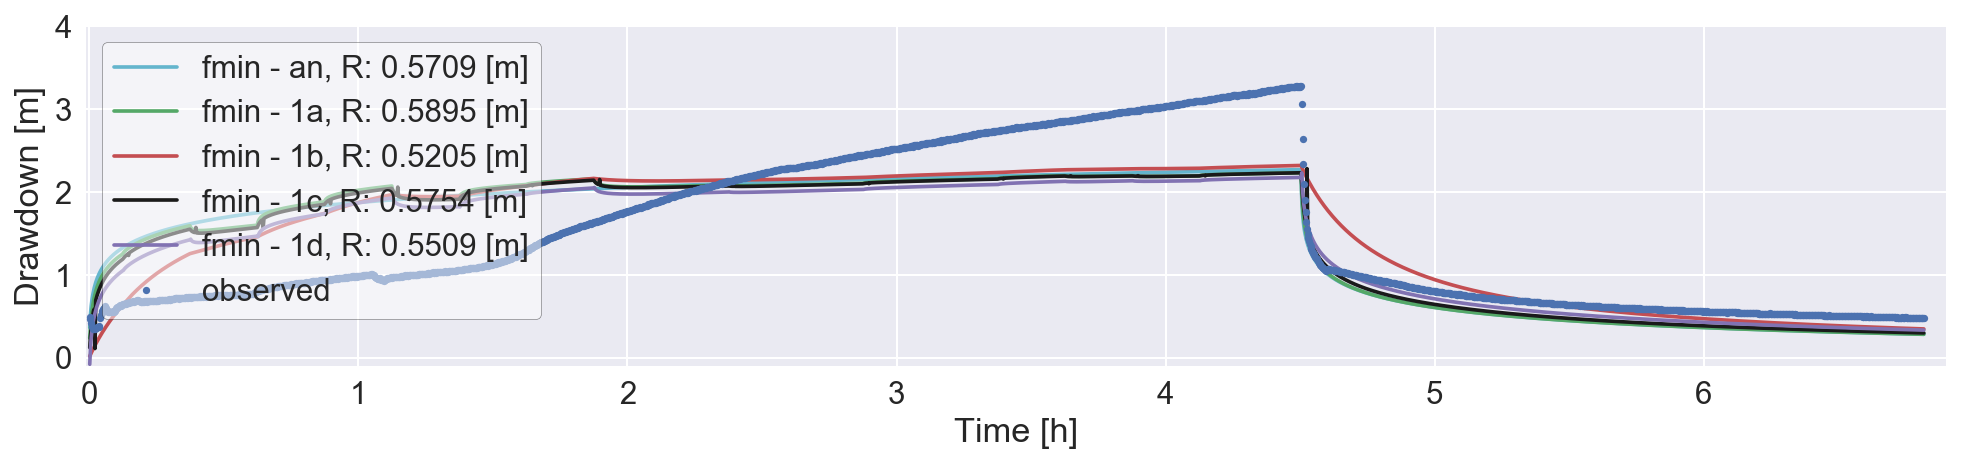
\includegraphics[width=\linewidth]{Janga2_1lay_fmin}
		\captionsetup{justification=centering}		
		\caption{\label{fig:Janga2_1lay_fmin}}
		\end{subfigure}\vfill
	\begin{subfigure}[b]{0.64\linewidth}
		\centering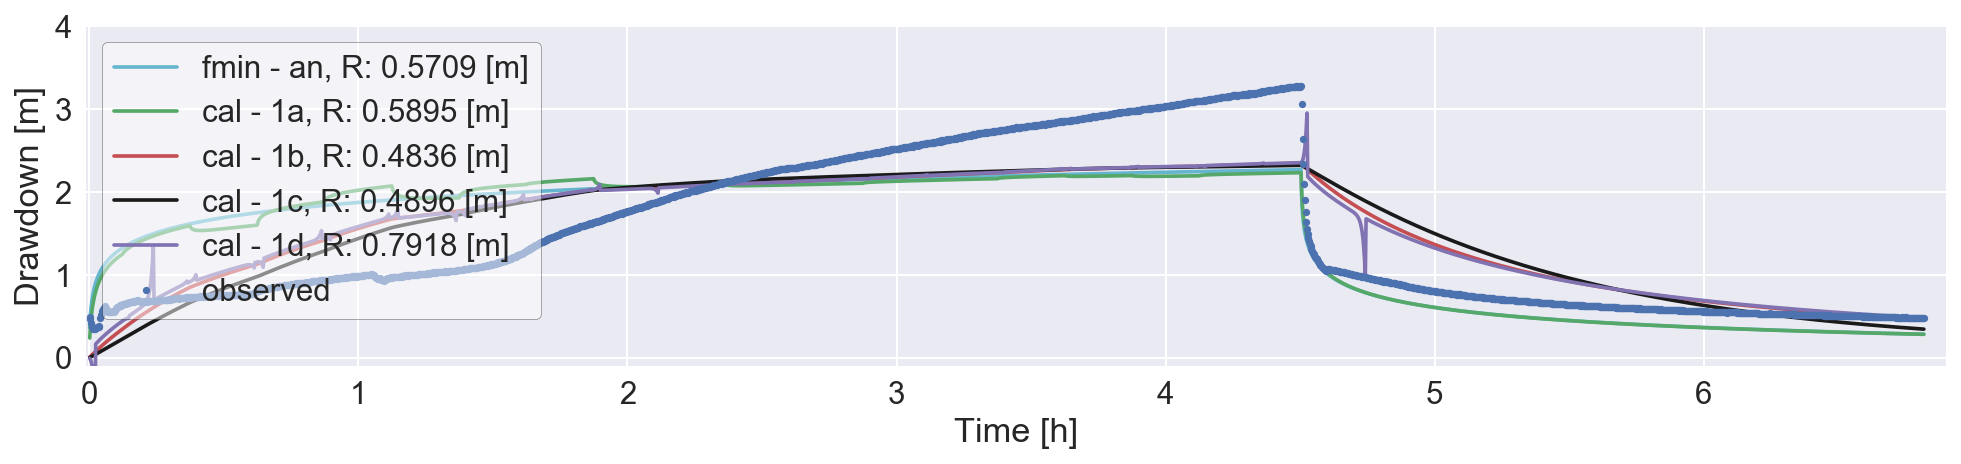
\includegraphics[width=\linewidth]{Janga2_1lay_cal}
		\captionsetup{justification=centering}		
		\caption{\label{fig:Janga2_1lay_cal}}
		\end{subfigure}
	\captionsetup{justification=centering}	
	\caption{Janga second attempt single layer fieldwork data analysis by the optimization (\subref{fig:Janga2_1lay_fmin}) fmin-RMSE method and (\subref{fig:Janga2_1lay_cal}) TTim calibration method} 
	\label{fig:Janga2_1lay_analysis}
\end{figure} 

\begin{figure}[h!]
	\centering
	\begin{subfigure}[b]{0.64\linewidth}
		\centering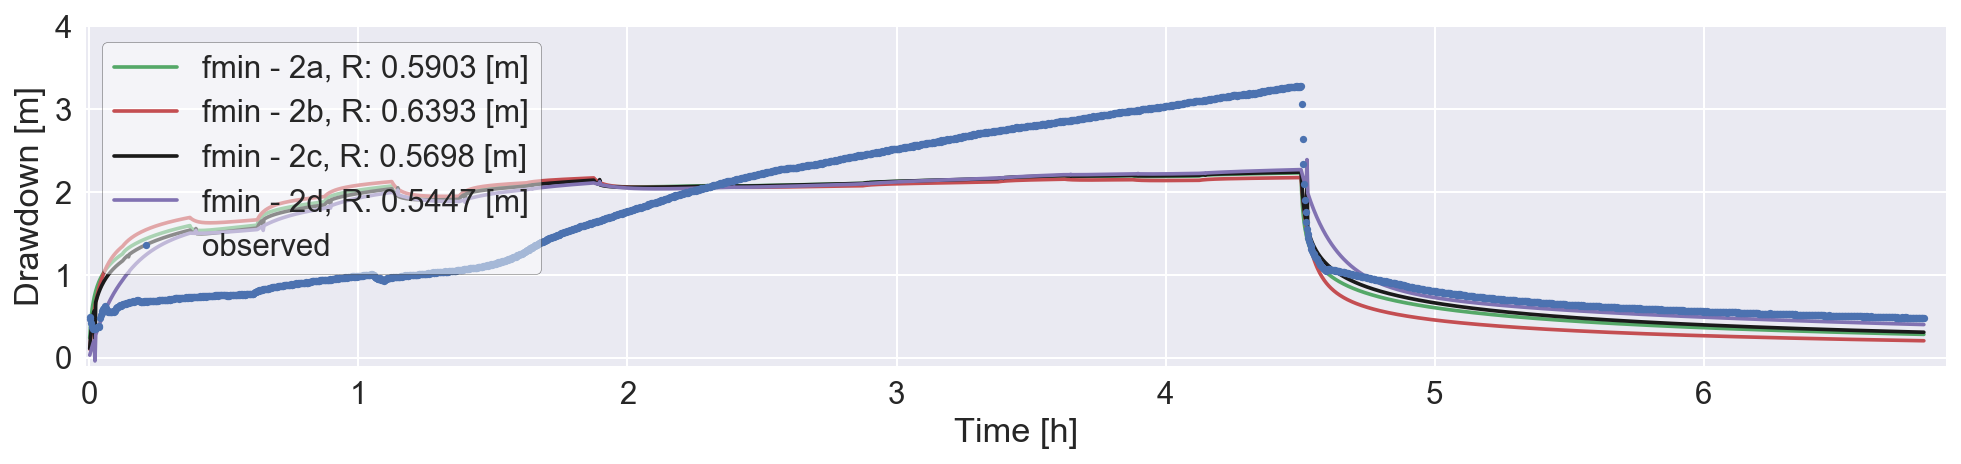
\includegraphics[width=\linewidth]{Janga2_2lay_fmin}
		\captionsetup{justification=centering}		
		\caption{\label{fig:Janga2_2lay_fmin}}
		\end{subfigure}\vfill
	\begin{subfigure}[b]{0.64\linewidth}
		\centering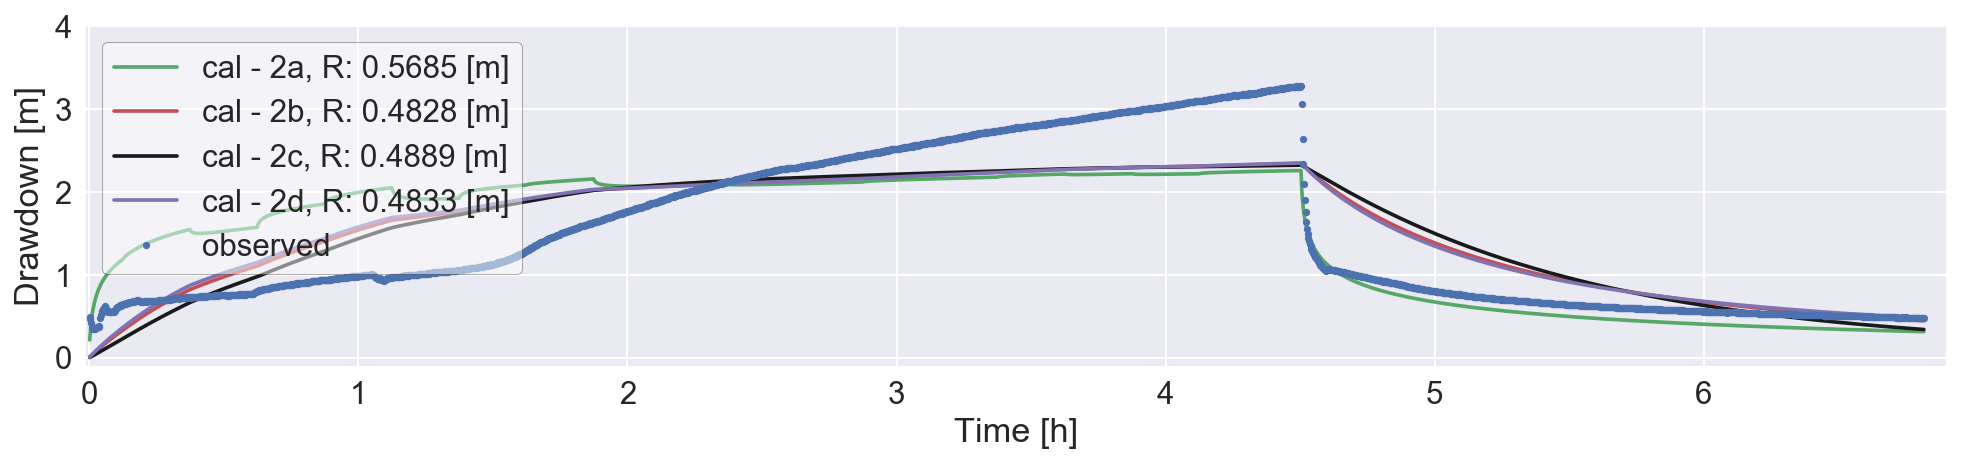
\includegraphics[width=\linewidth]{Janga2_2lay_cal}
		\captionsetup{justification=centering}		
		\caption{\label{fig:Janga2_2lay_cal}}
		\end{subfigure}
	\captionsetup{justification=centering}	
	\caption{Janga second attempt double layer fieldwork data analysis by the optimization (\subref{fig:Janga2_2lay_fmin}) fmin-RMSE method and (\subref{fig:Janga2_2lay_cal}) TTim calibration method} 
	\label{fig:Janga2_2lay_analysis}
\end{figure} 

\begin{figure}[h!]
	\centering
	\begin{subfigure}[b]{0.64\linewidth}
		\centering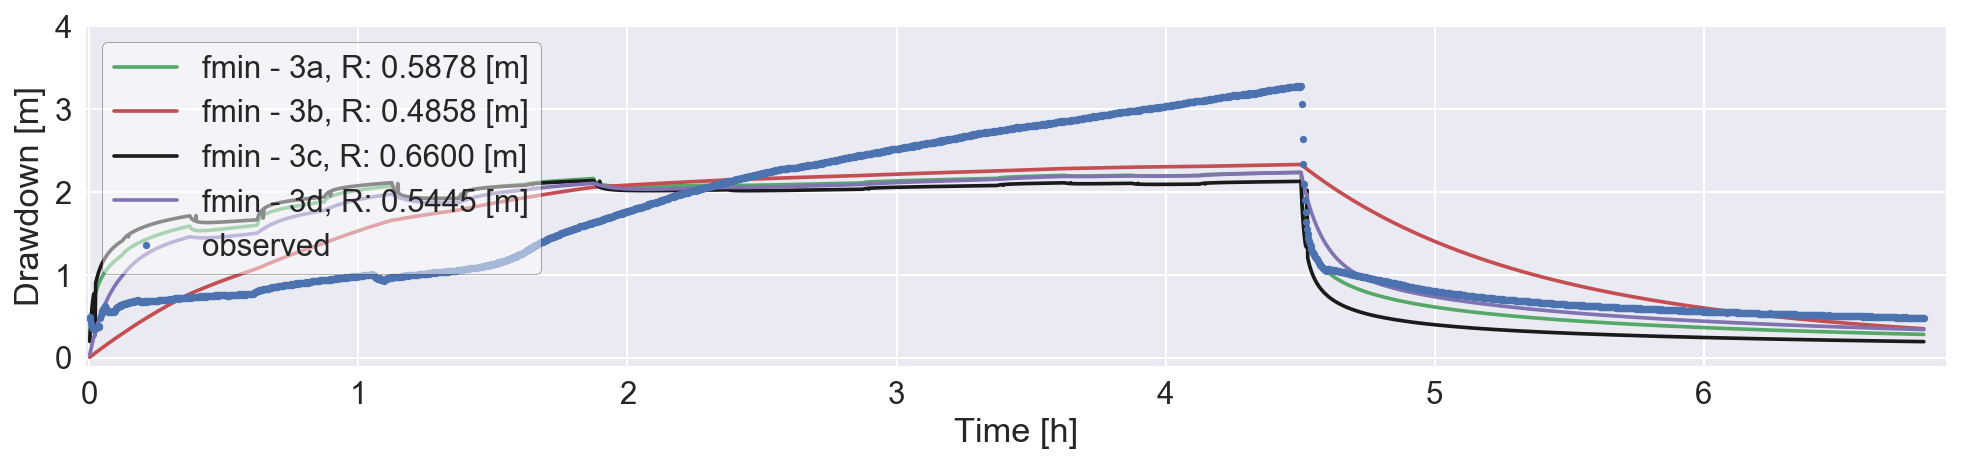
\includegraphics[width=\linewidth]{Janga2_3lay_fmin}
		\captionsetup{justification=centering}		
		\caption{\label{fig:Janga2_3lay_fmin}}
		\end{subfigure}\vfill
	\begin{subfigure}[b]{0.64\linewidth}
		\centering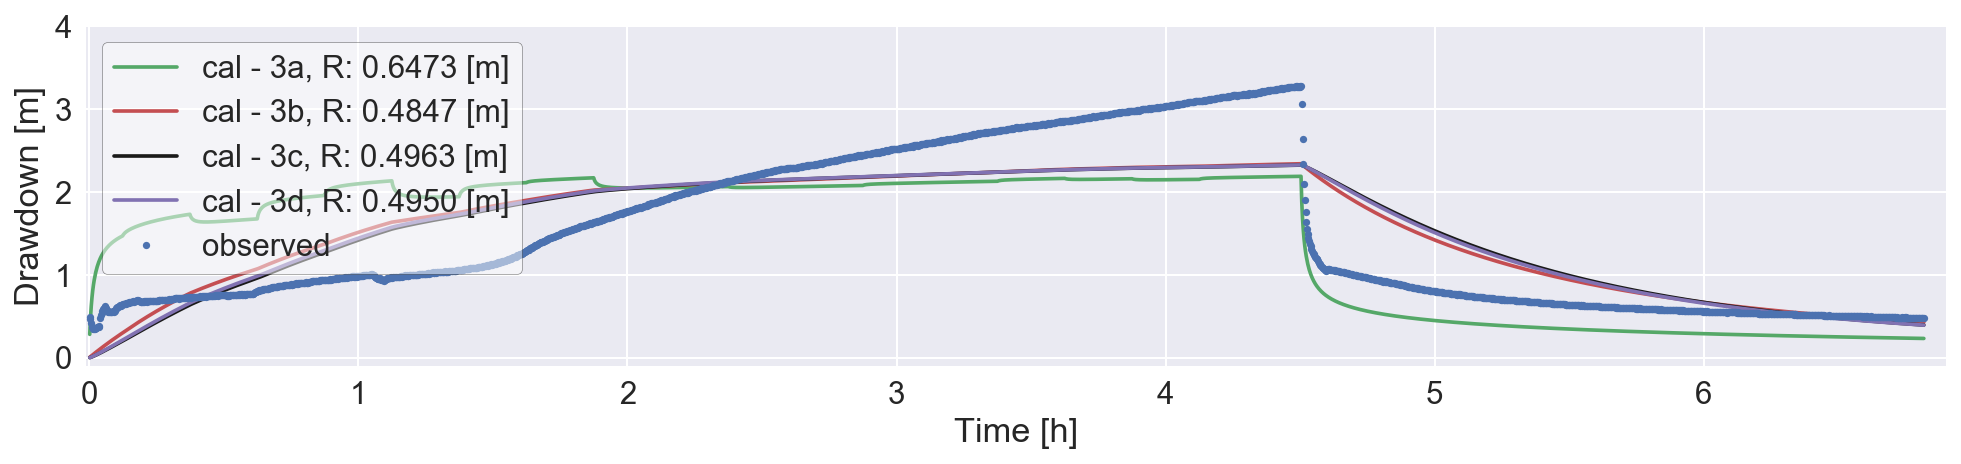
\includegraphics[width=\linewidth]{Janga2_3lay_cal}
		\captionsetup{justification=centering}		
		\caption{\label{fig:Janga2_3lay_cal}}
		\end{subfigure}
	\captionsetup{justification=centering}	
	\caption{Janga second attempt partially penetrating double layer fieldwork data analysis by the optimization (\subref{fig:Janga2_3lay_fmin}) fmin-RMSE method and (\subref{fig:Janga2_3lay_cal}) TTim calibration method} 
	\label{fig:Janga2_3lay_analysis}
\end{figure} 

\clearpage

\begin{figure}[h!]
	\centering
	\begin{subfigure}[b]{\linewidth}
		\centering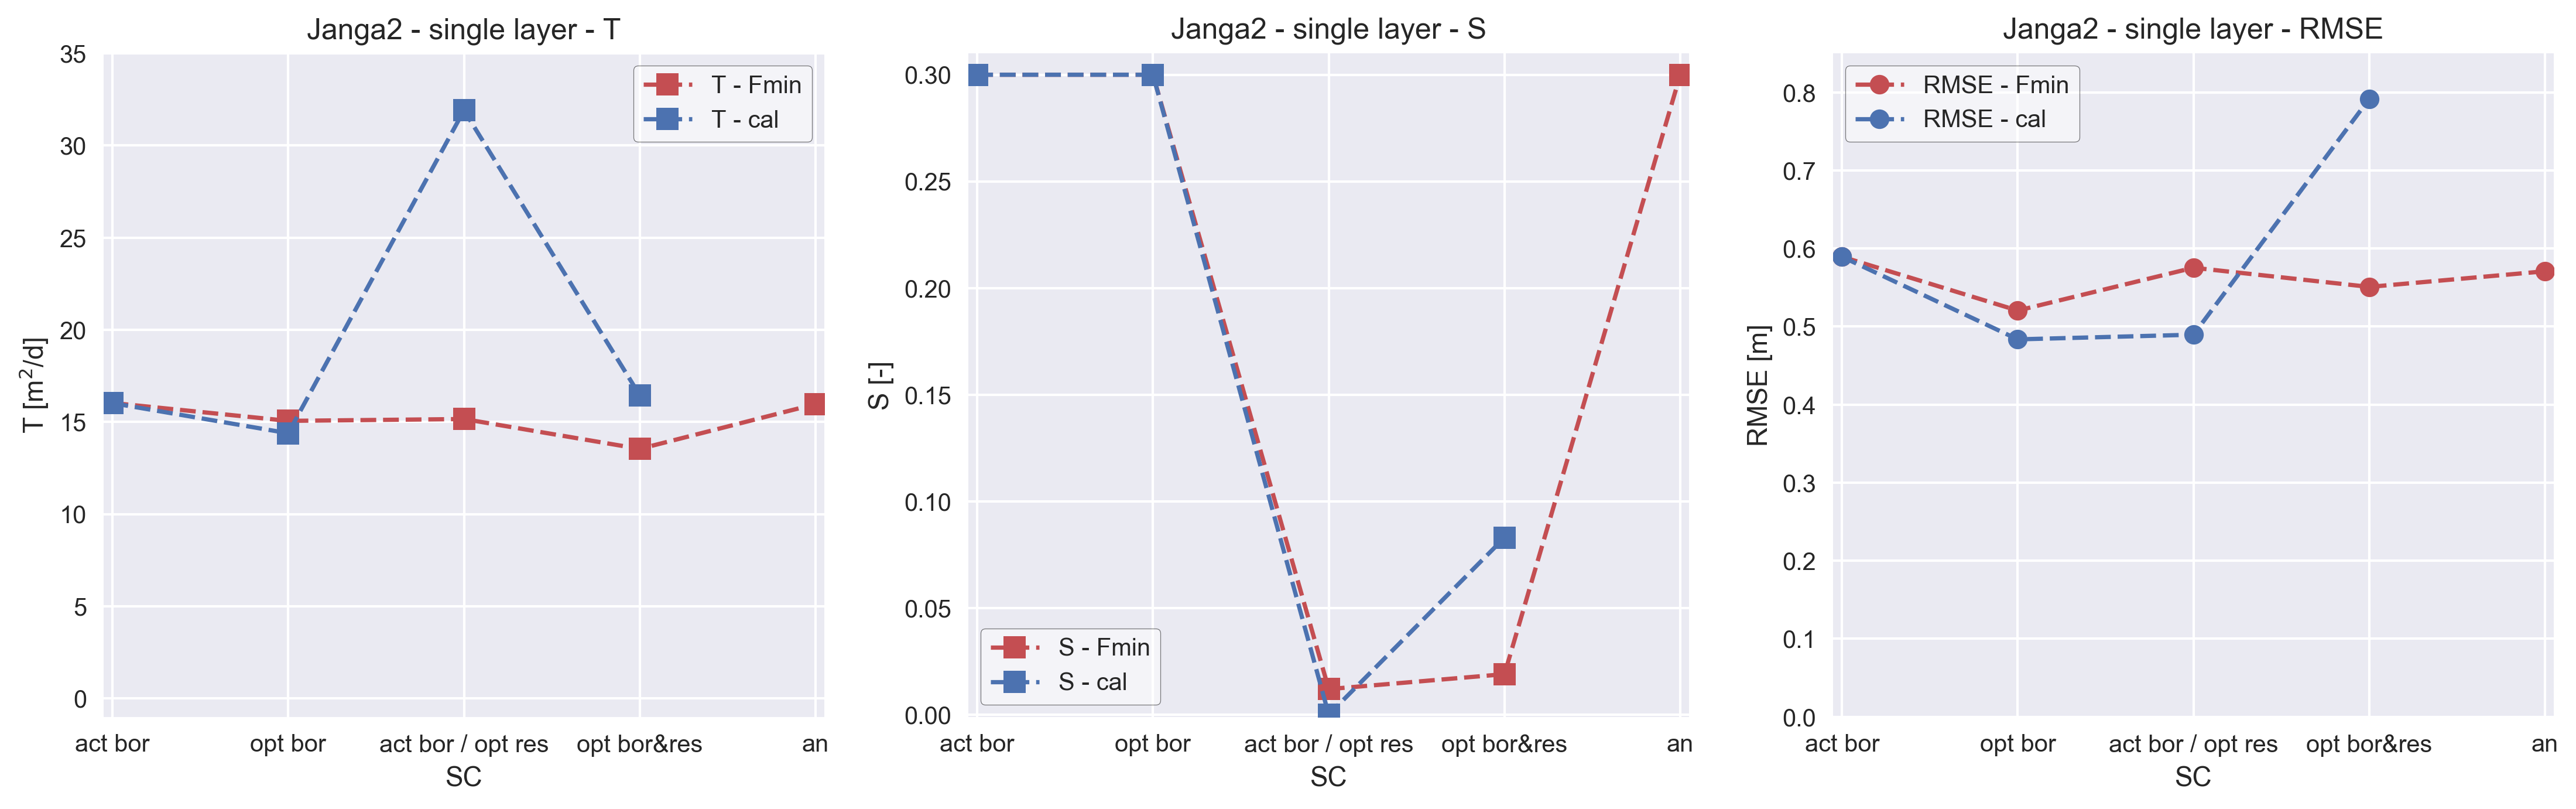
\includegraphics[width=\linewidth]{J2_para_results_1lay}
		\captionsetup{justification=centering}		
		\caption{\label{fig:J2_para_results_1lay}}
		\end{subfigure}\vfill
	\begin{subfigure}[b]{\linewidth}
		\centering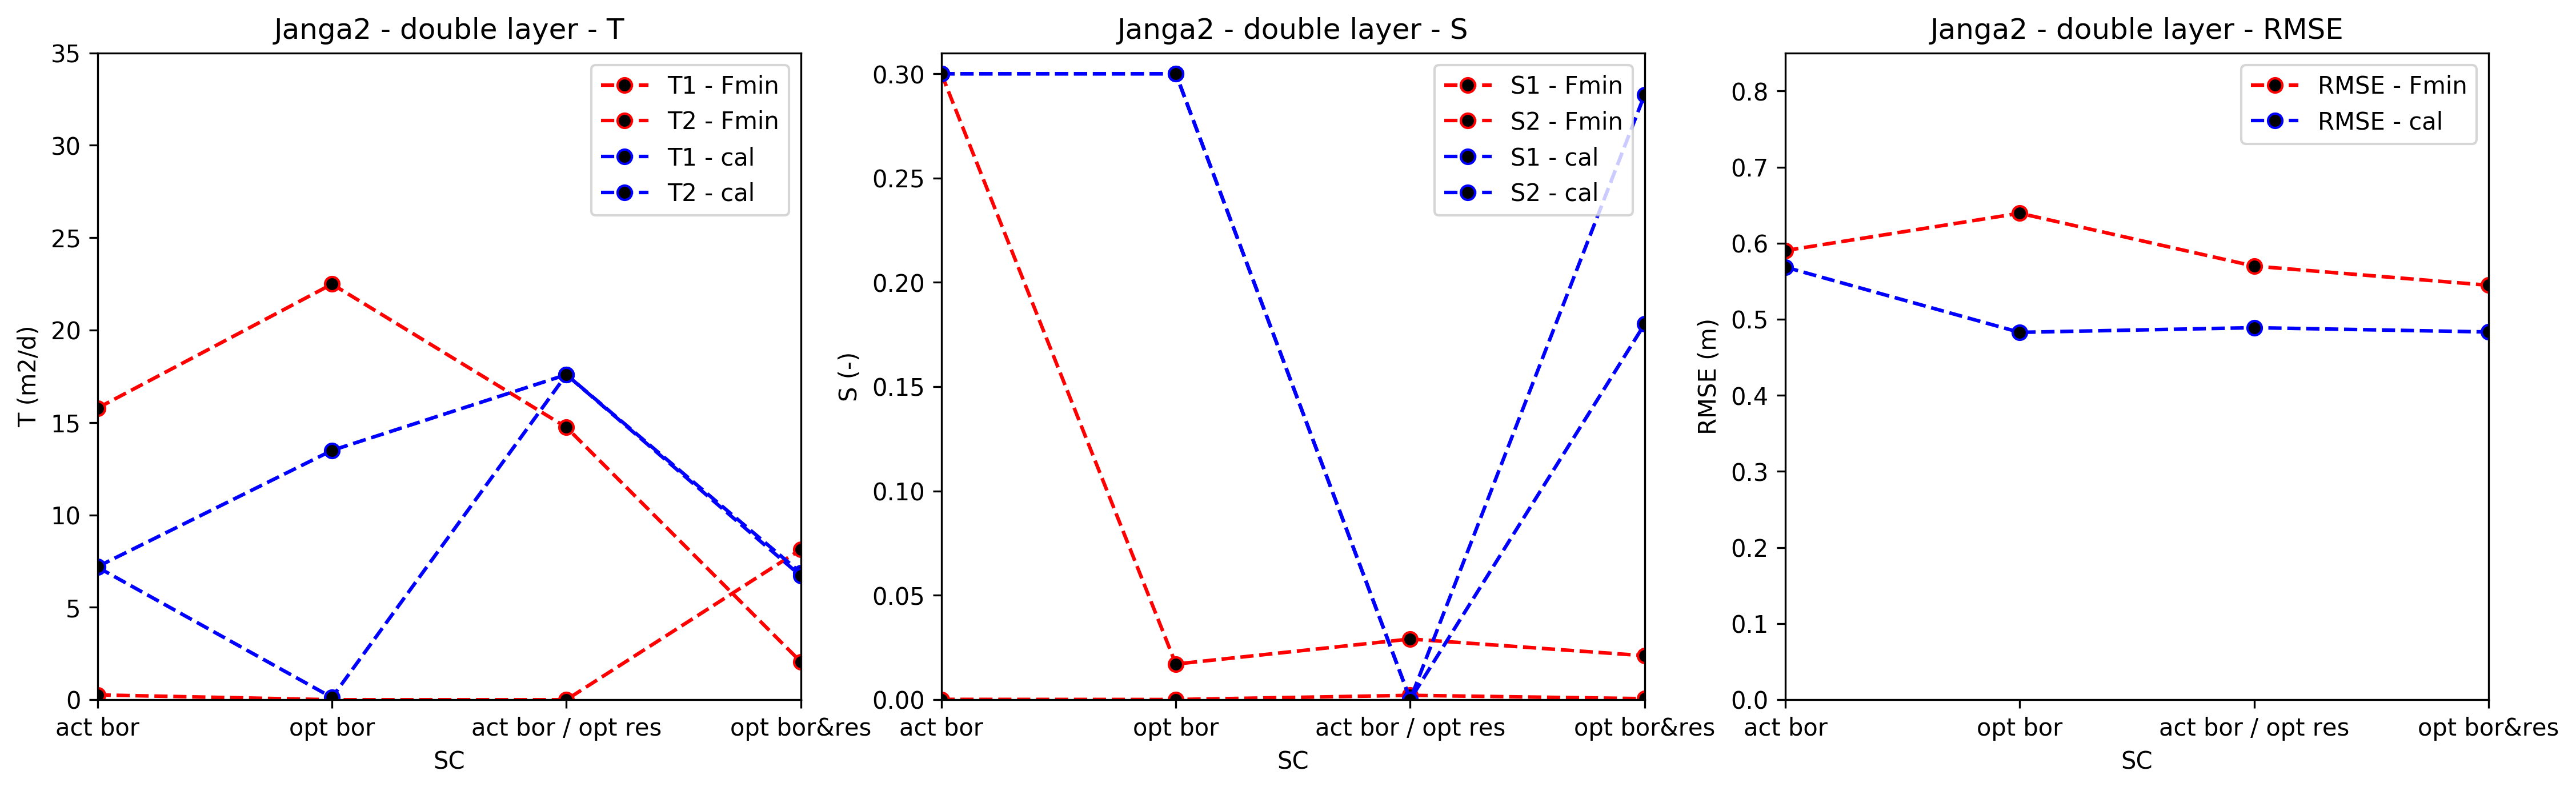
\includegraphics[width=\linewidth]{J2_para_results_2lay}
		\captionsetup{justification=centering}		
		\caption{\label{fig:J2_para_results_2lay}}
		\end{subfigure}
	\begin{subfigure}[b]{\linewidth}
		\centering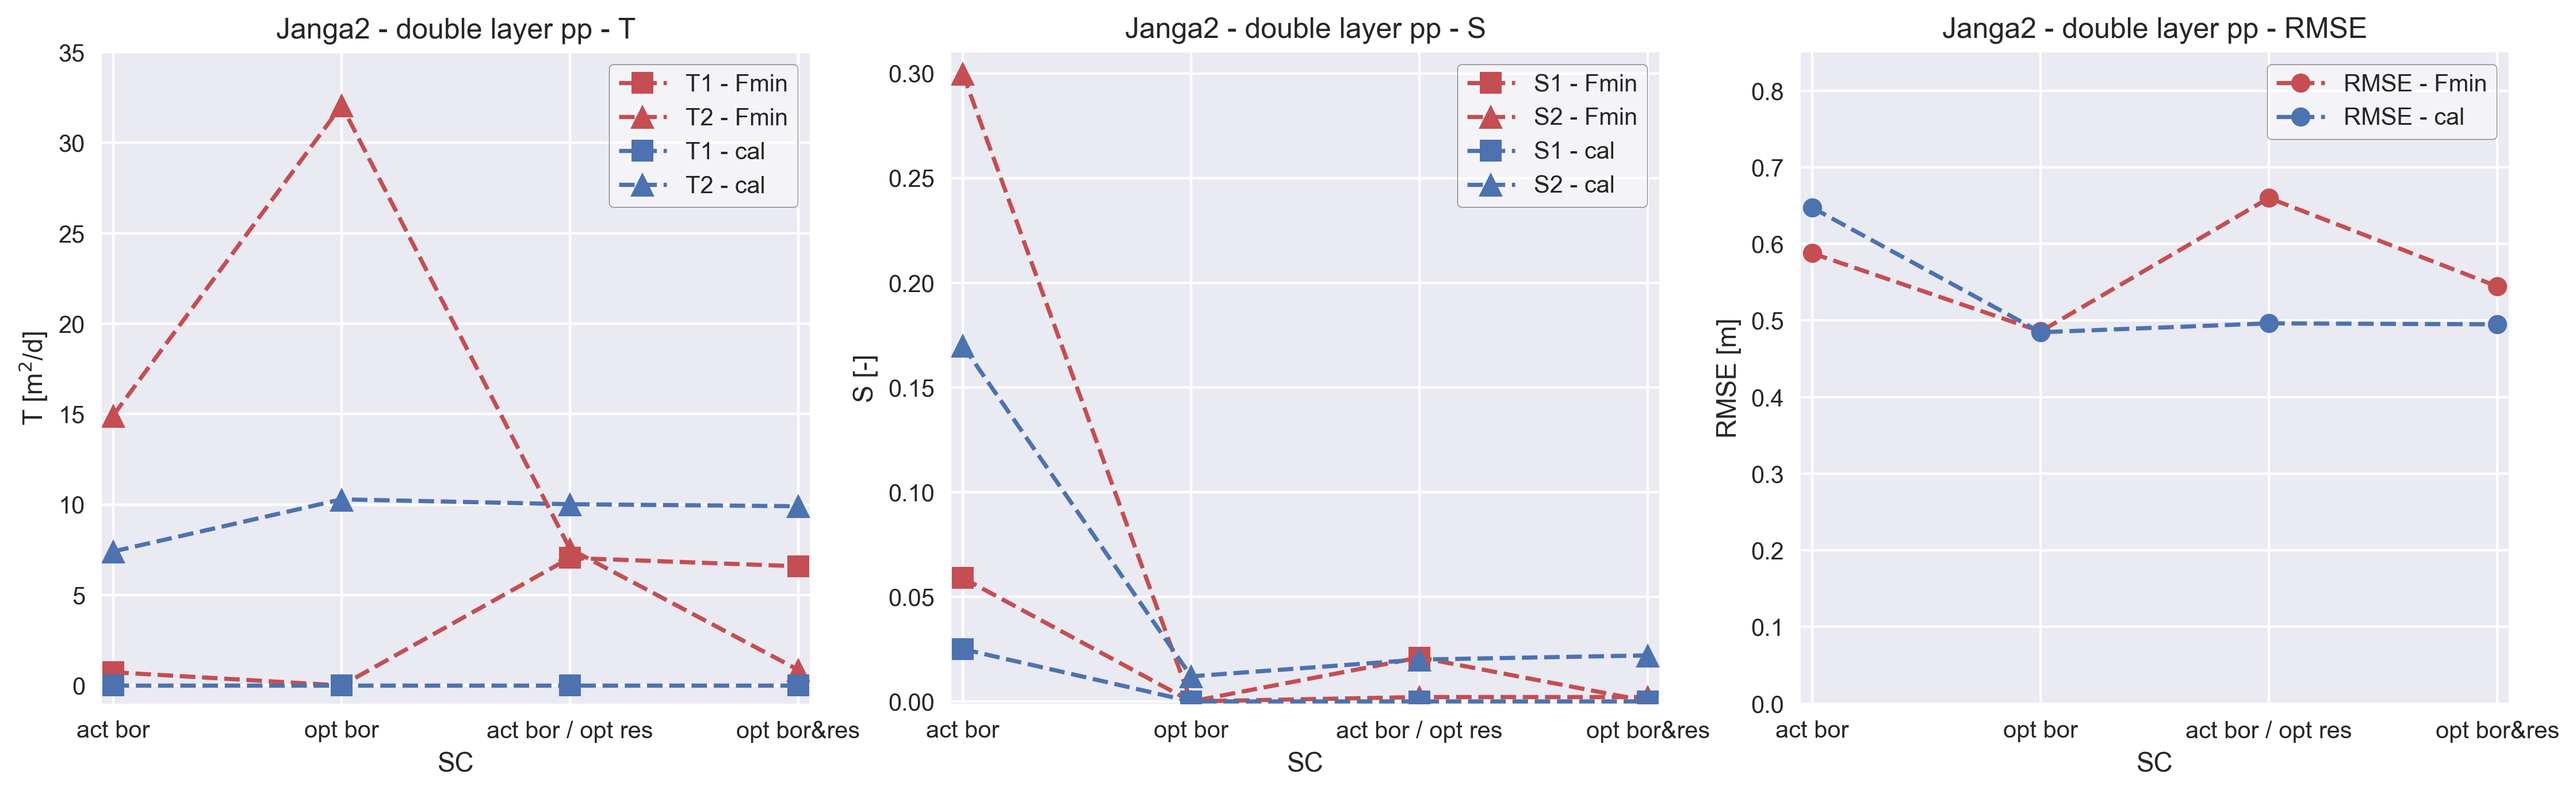
\includegraphics[width=\linewidth]{J2_para_results_3lay}
		\captionsetup{justification=centering}		
		\caption{\label{fig:J2_para_results_3lay}}
		\end{subfigure}		
	\captionsetup{justification=centering}	
	\caption{Janga second attempt - overview determined (Fmin and Cal) optimal parameter values of (\subref{fig:fig:J2_para_results_1lay}) a single layer system, (\subref{fig:fig:J2_para_results_2lay}) a double layer system, and (\subref{fig:fig:J2_para_results_3lay}) a system with two layers and partial penetration of the well} 
	\label{fig:J2_para_results}
\end{figure} 


\clearpage\section{Ziong - overview}
\label{sec:Ziong_overview}

\begin{figure}[h!]
	\centering
	\begin{subfigure}[b]{0.65\linewidth}
		\centering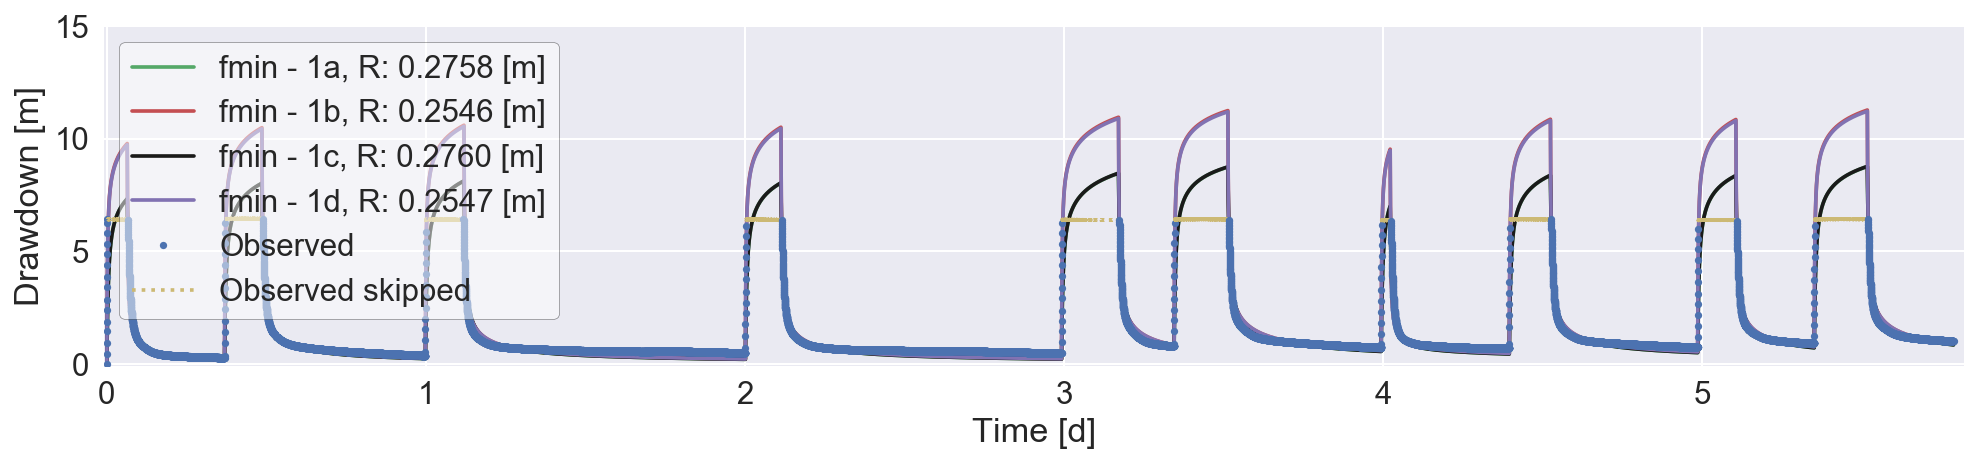
\includegraphics[width=\linewidth]{Ziong_1lay_fmin}
		\captionsetup{justification=centering}		
		\caption{\label{fig:Ziong_1lay_fmin}}
		\end{subfigure}\vfill
	\begin{subfigure}[b]{0.65\linewidth}
		\centering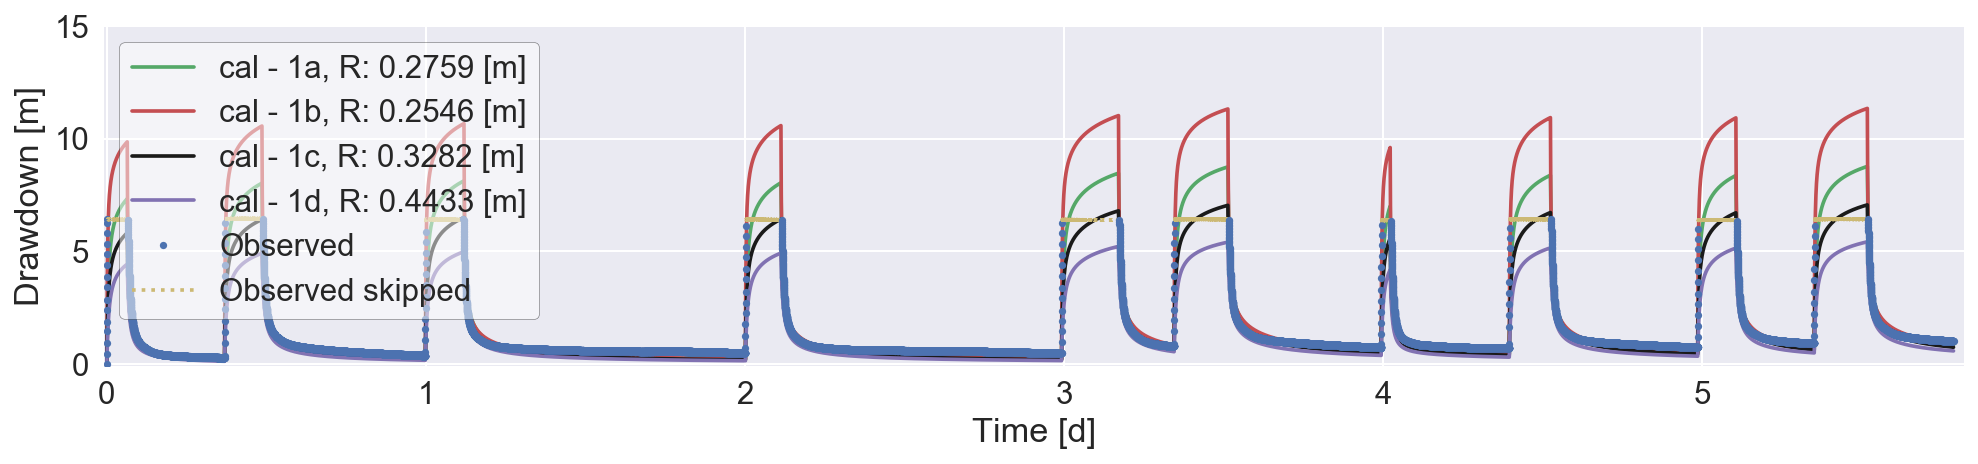
\includegraphics[width=\linewidth]{Ziong_1lay_cal}
		\captionsetup{justification=centering}		
		\caption{\label{fig:Ziong_1lay_cal}}
		\end{subfigure}
	\captionsetup{justification=centering}	
	\caption{Ziong single layer fieldwork data analysis by the optimization (\subref{fig:Ziong_1lay_fmin}) fmin-RMSE method and (\subref{fig:Ziong_1lay_cal}) TTim calibration method} 
	\label{fig:Ziong_1lay_analysis}
\end{figure} 

\begin{figure}[h!]
	\centering
	\begin{subfigure}[b]{0.65\linewidth}
		\centering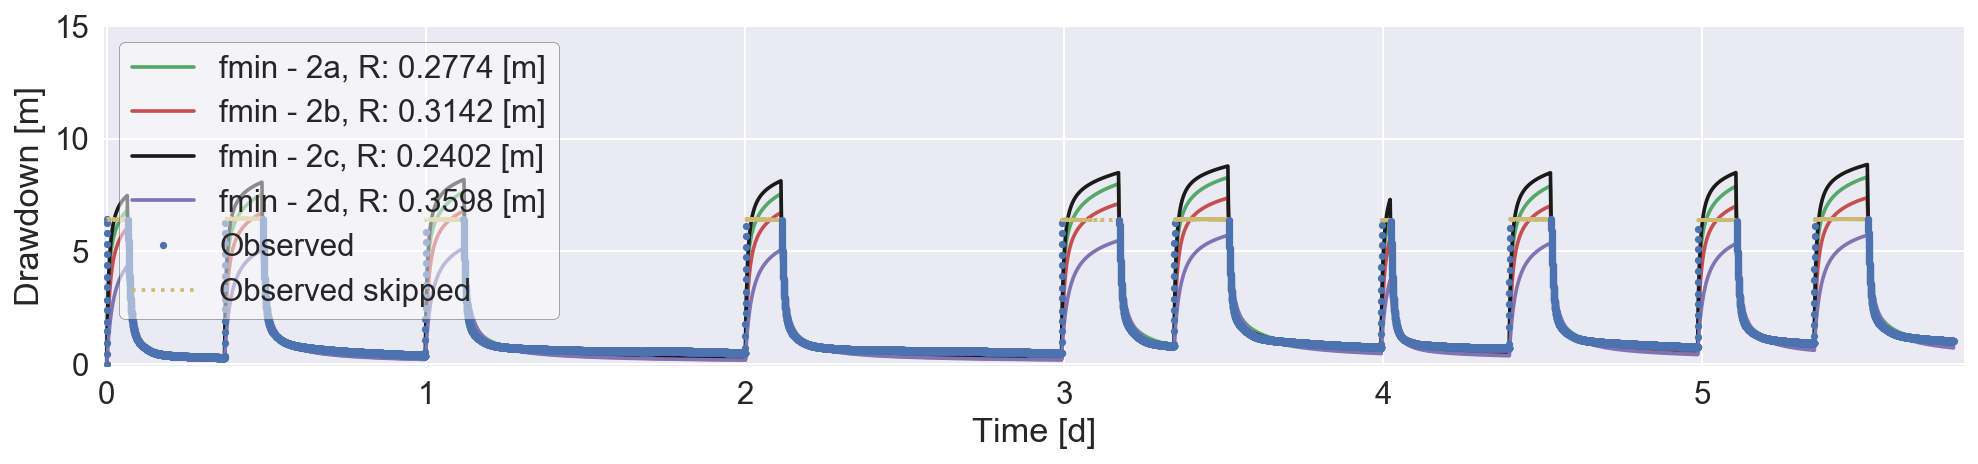
\includegraphics[width=\linewidth]{Ziong_2lay_fmin}
		\captionsetup{justification=centering}		
		\caption{\label{fig:Ziong_2lay_fmin}}
		\end{subfigure}\vfill
	\begin{subfigure}[b]{0.65\linewidth}
		\centering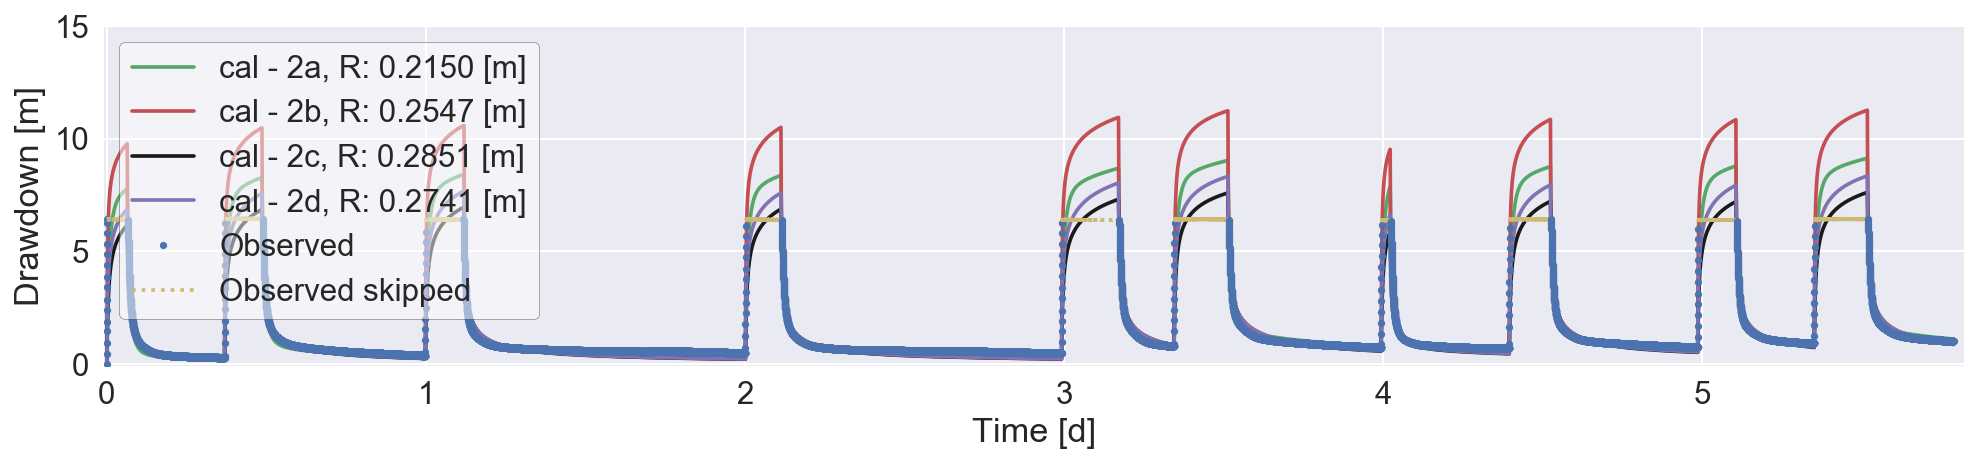
\includegraphics[width=\linewidth]{Ziong_2lay_cal}
		\captionsetup{justification=centering}		
		\caption{\label{fig:Ziong_2lay_cal}}
		\end{subfigure}
	\captionsetup{justification=centering}	
	\caption{Ziong double layer fieldwork data analysis by the optimization (\subref{fig:Ziong_2lay_fmin}) fmin-RMSE method and (\subref{fig:Ziong_2lay_cal}) TTim calibration method} 
	\label{fig:Ziong_2lay_analysis}
\end{figure} 

\begin{figure}[h!]
	\centering
	\begin{subfigure}[b]{0.65\linewidth}
		\centering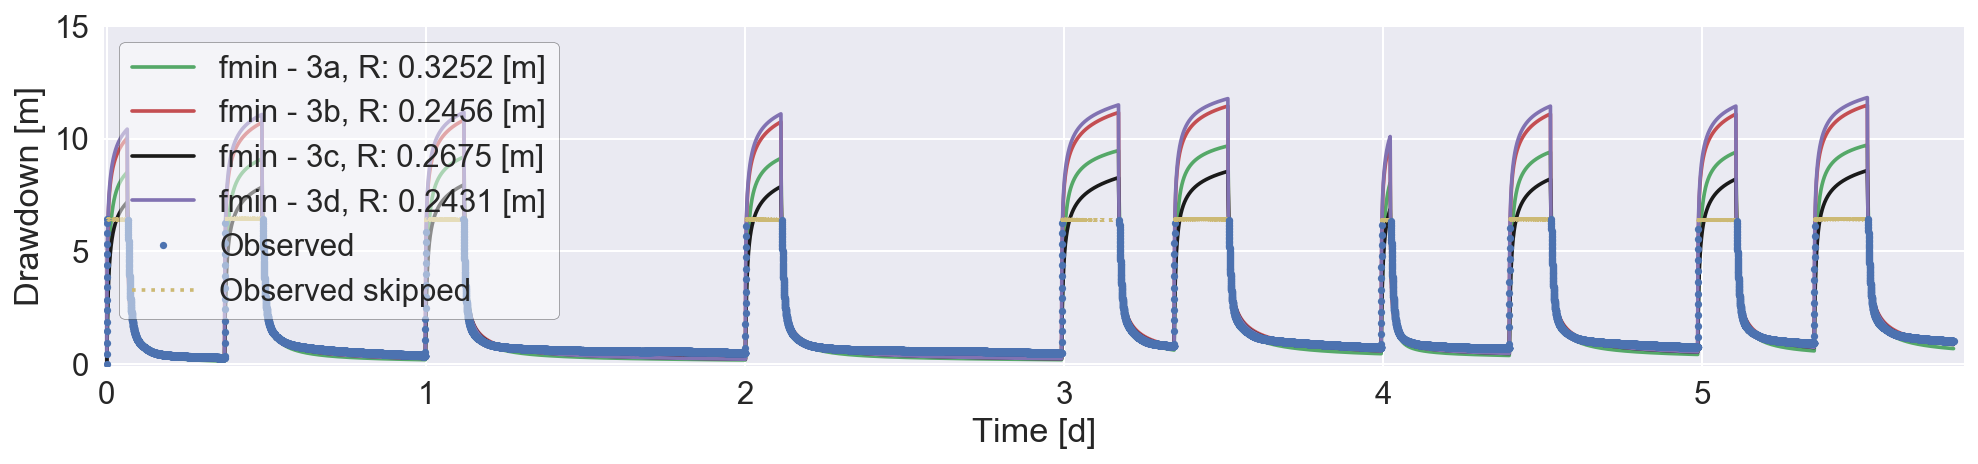
\includegraphics[width=\linewidth]{Ziong_3lay_fmin}
		\captionsetup{justification=centering}		
		\caption{\label{fig:Ziong_3lay_fmin}}
		\end{subfigure}\vfill
	\begin{subfigure}[b]{0.65\linewidth}
		\centering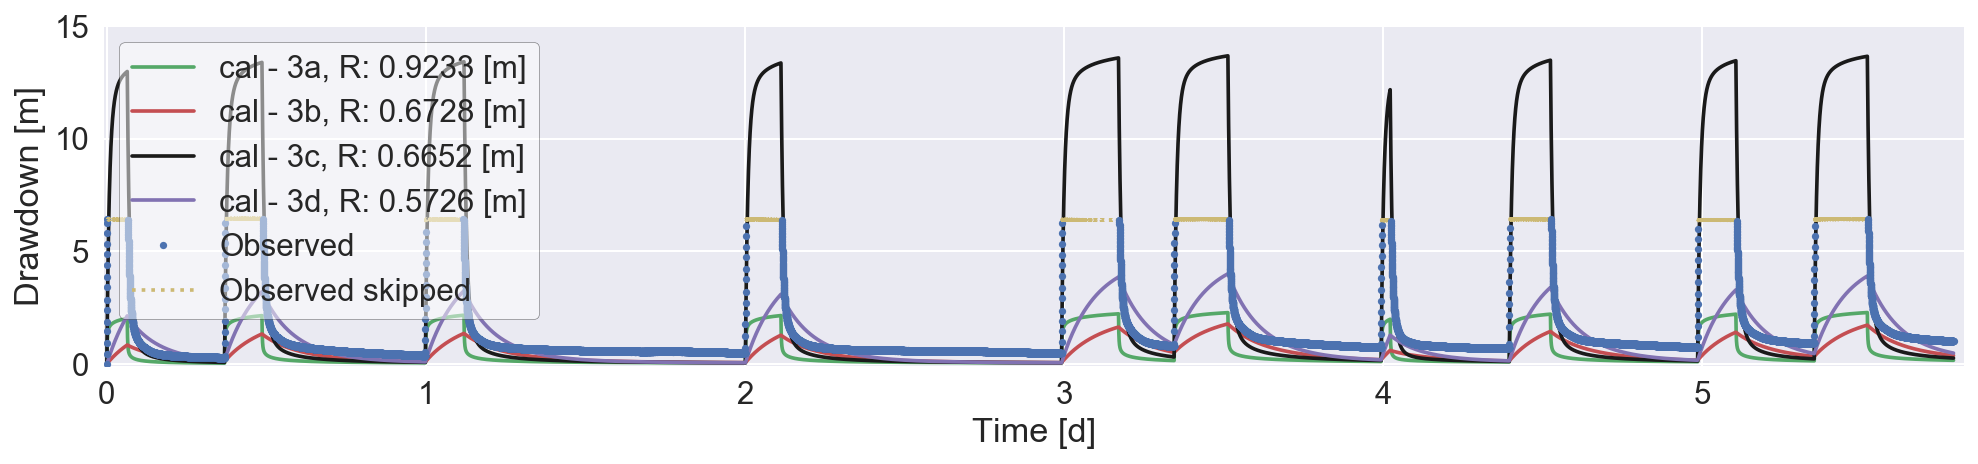
\includegraphics[width=\linewidth]{Ziong_3lay_cal}
		\captionsetup{justification=centering}		
		\caption{\label{fig:Ziong_3lay_cal}}
		\end{subfigure}
	\captionsetup{justification=centering}	
	\caption{Ziong partially penetrating double layer fieldwork data analysis by the optimization (\subref{fig:Ziong_3lay_fmin}) fmin-RMSE method and (\subref{fig:Ziong_3lay_cal}) TTim calibration method} 
	\label{fig:Ziong_3lay_analysis}
\end{figure} 

\clearpage

\begin{figure}[h!]
	\centering
	\begin{subfigure}[b]{\linewidth}
		\centering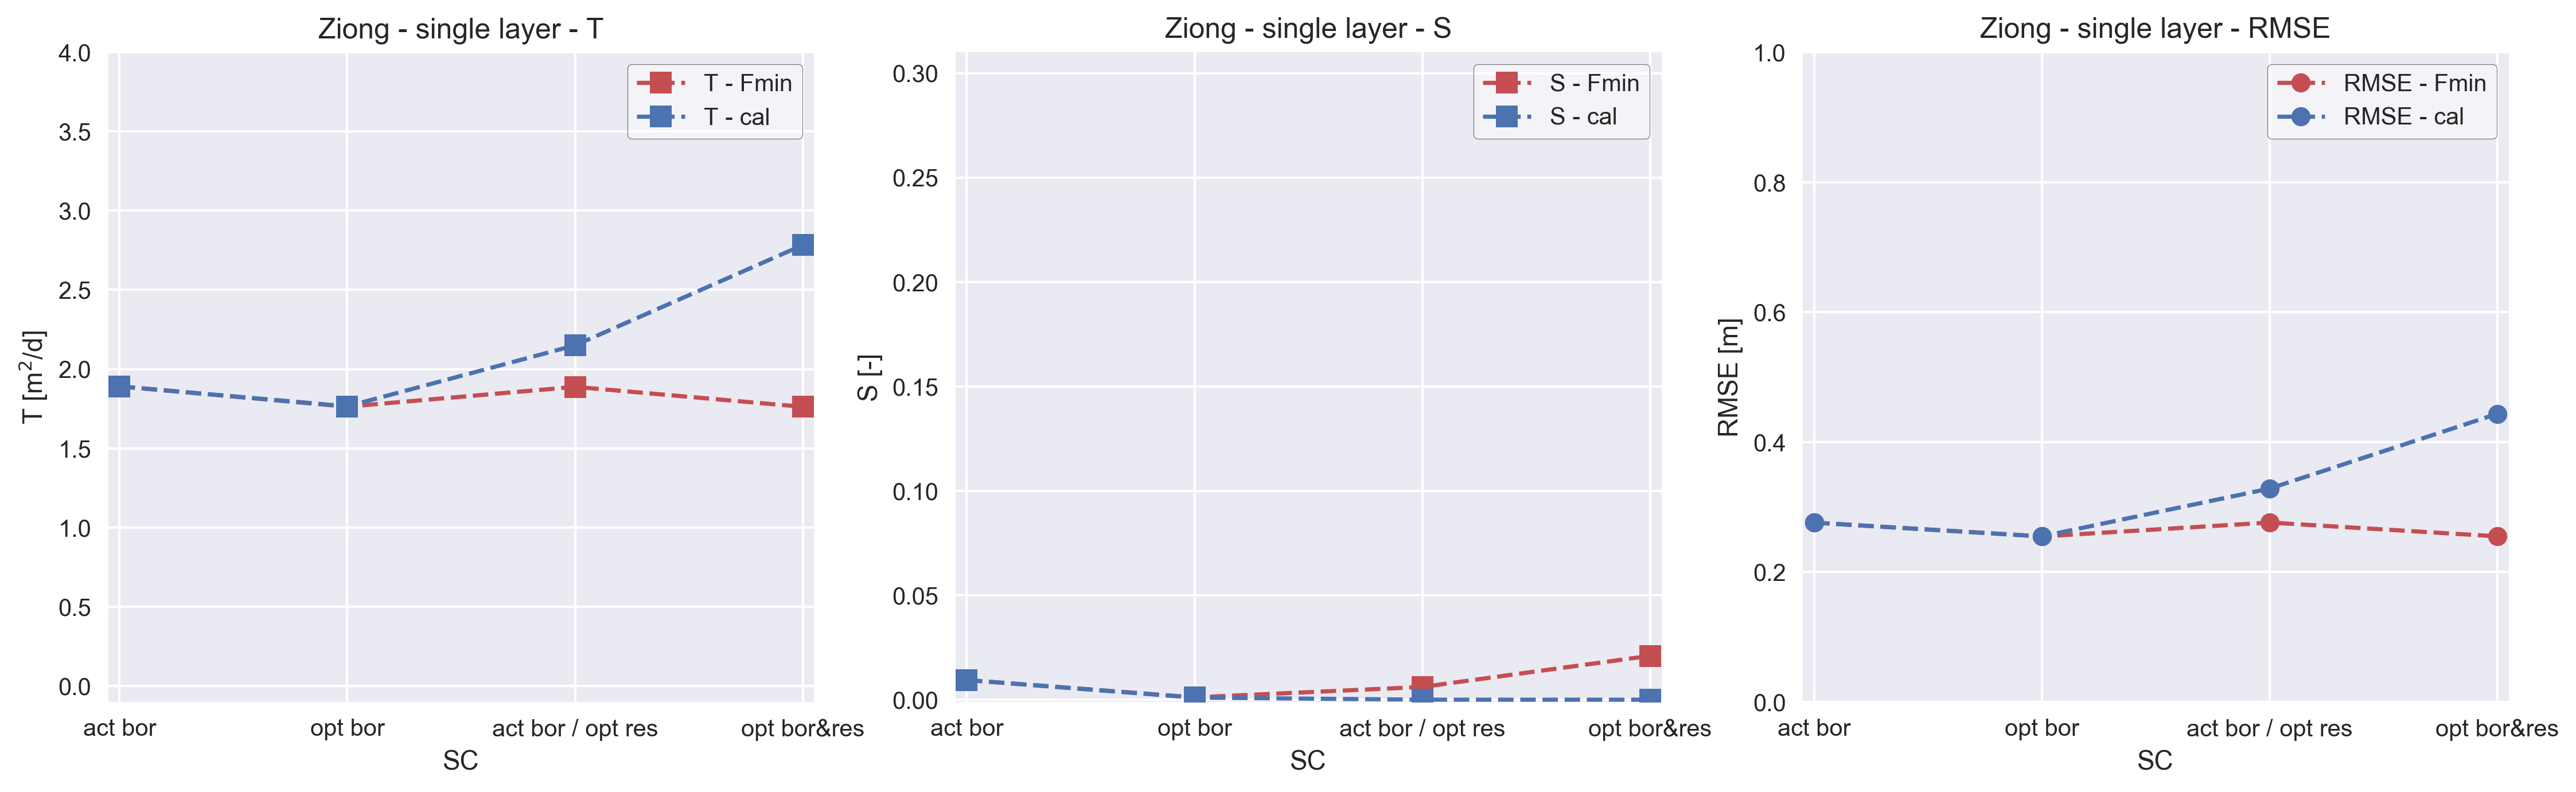
\includegraphics[width=\linewidth]{Ziong_para_results_1lay}
		\captionsetup{justification=centering}		
		\caption{\label{fig:Ziong_para_results_1lay}}
		\end{subfigure}\vfill
	\begin{subfigure}[b]{\linewidth}
		\centering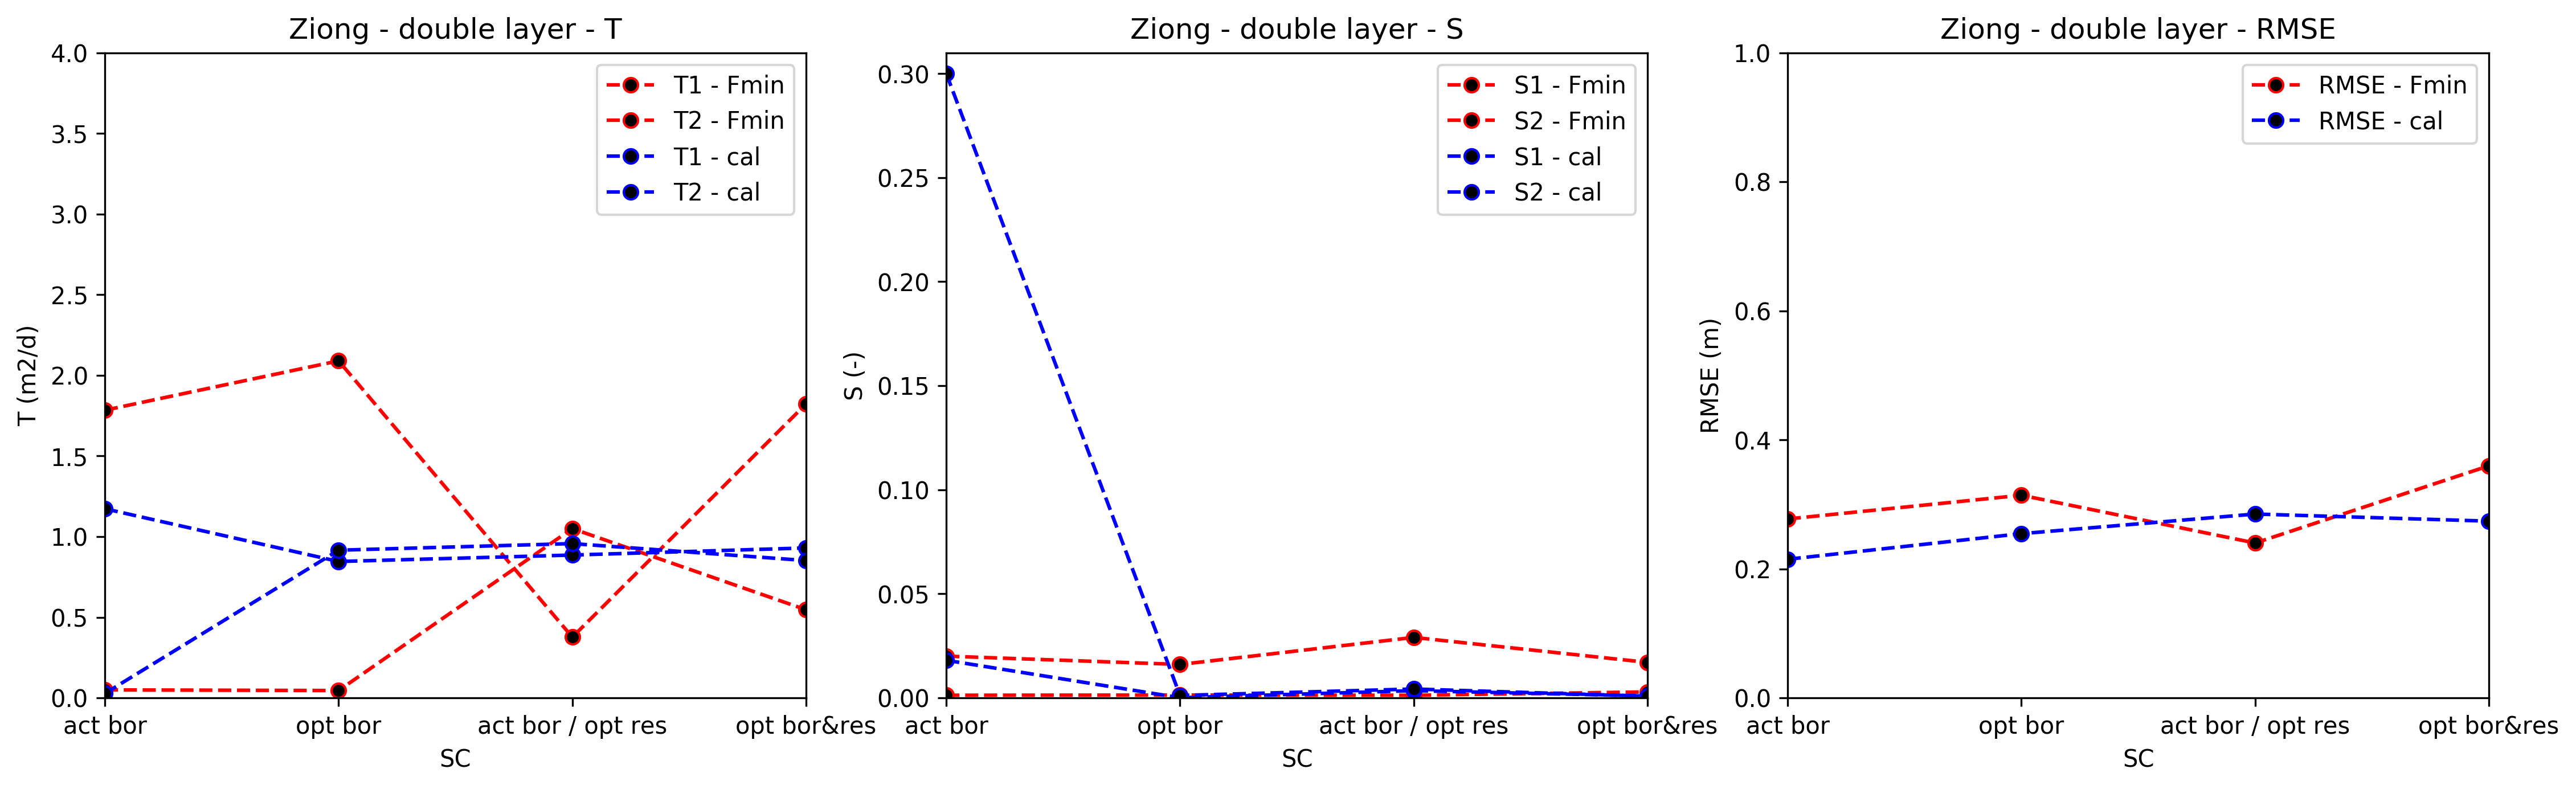
\includegraphics[width=\linewidth]{Ziong_para_results_2lay}
		\captionsetup{justification=centering}		
		\caption{\label{fig:Ziong_para_results_2lay}}
		\end{subfigure}
	\begin{subfigure}[b]{\linewidth}
		\centering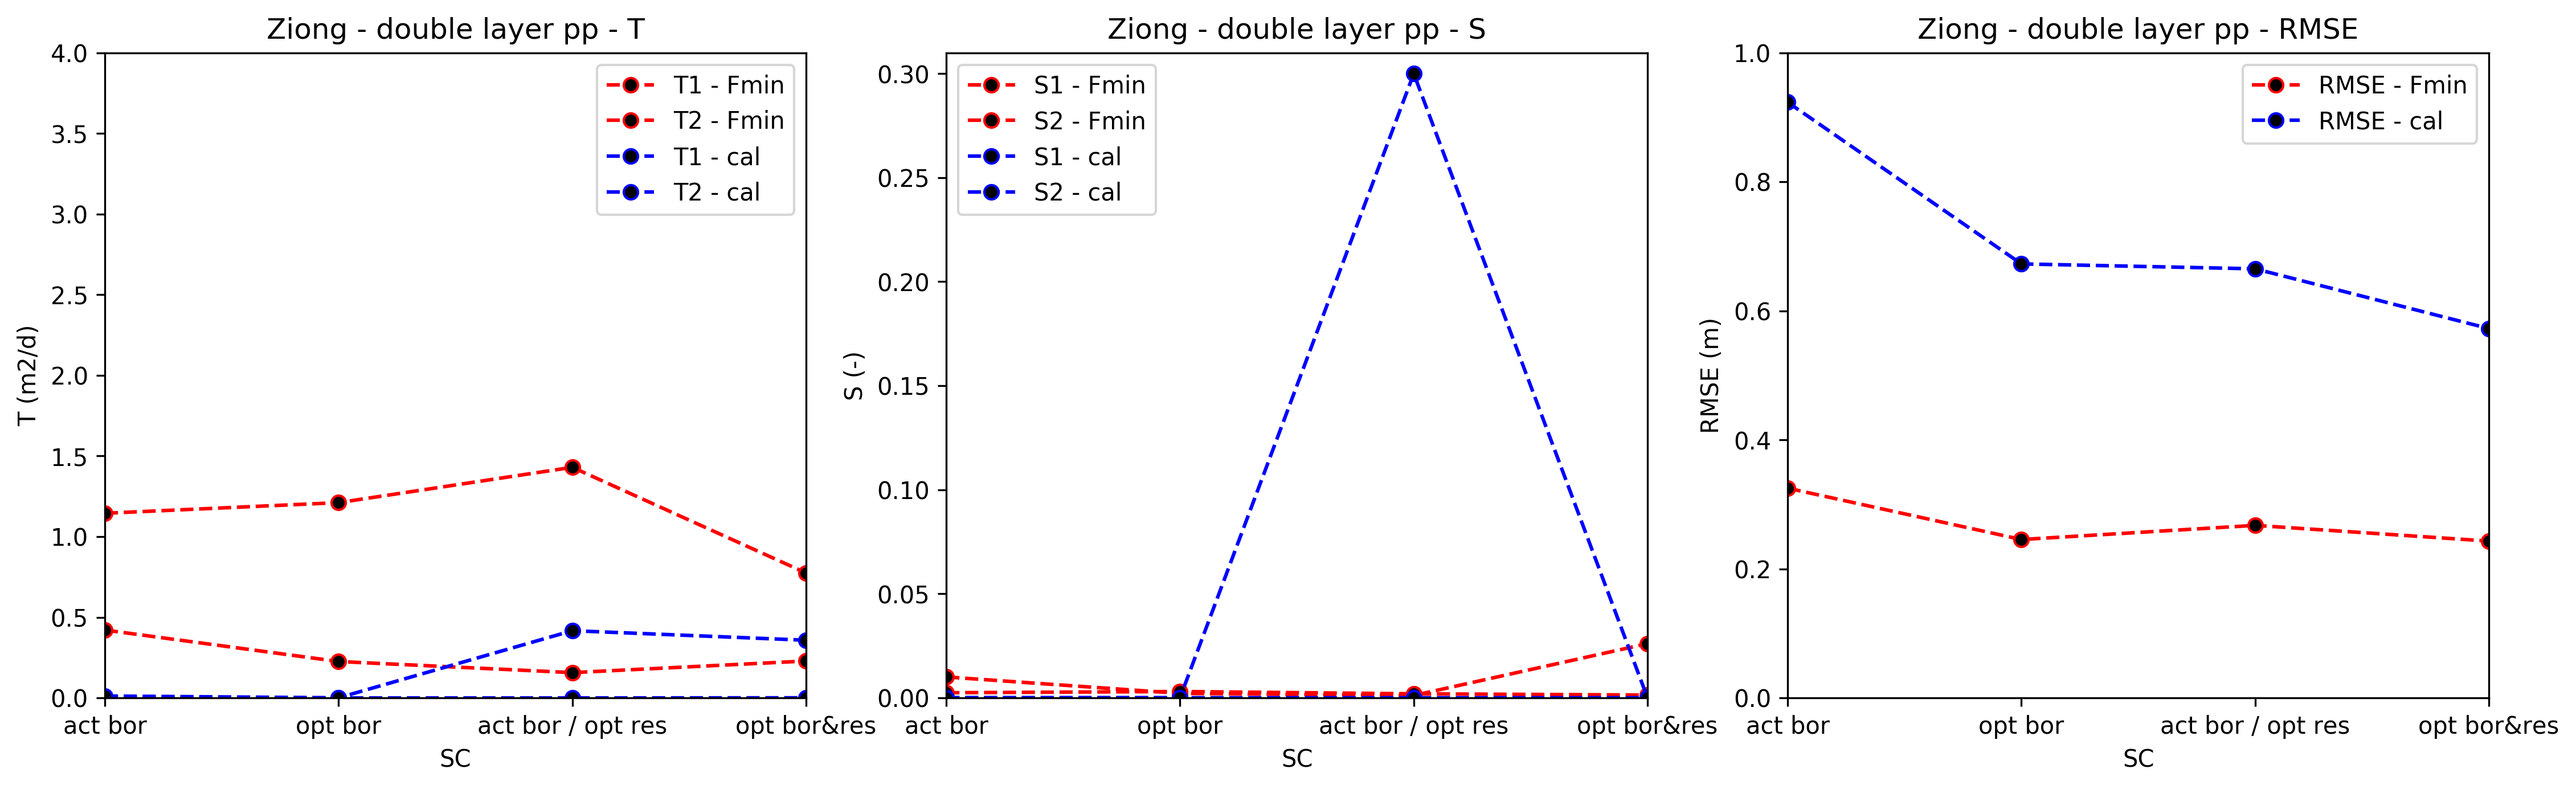
\includegraphics[width=\linewidth]{Ziong_para_results_3lay}
		\captionsetup{justification=centering}		
		\caption{\label{fig:Ziong_para_results_3lay}}
		\end{subfigure}		
	\captionsetup{justification=centering}	
	\caption{Ziong - overview determined (Fmin and Cal) optimal parameter values of (\subref{fig:fig:Ziong_para_results_1lay}) a single layer system, (\subref{fig:fig:Ziong_para_results_2lay}) a double layer system, and (\subref{fig:fig:Ziong_para_results_3lay}) a system with two layers and partial penetration of the well} 
	\label{fig:Ziong_para_results}
\end{figure} 
